%% Master: ../rough_volterra_lognormal.tex. Generated by make_qf_version.py: edit the master and regenerate, do not edit this file.
%% Quantitative Finance (rQUF2e) version of rough_volterra_lognormal_sv.tex, derived by
%% make_qf_version.py from the master draft (its revision date is in the master's header). Layout only:
%% no prose or mathematics was changed. The working draft stays the master; regenerate this file after editing it.
%% Location: paper/qf/ (figures are read from ../figures/). Compile: pdflatex -> bibtex -> pdflatex -> pdflatex;
%% rQUF2e.cls and rQUF.bst (from the journal's rquflatex.zip) sit in this folder.
%% Journal rules applied (rQUFguide.tex v2.1): class without options, no geometry package, natbib
%% author-date loaded by the class, \tbl{}{} table captions above the body, figure captions below,
%% no float placement specifiers, references before the appendices, \appendices for the appendix
%% sections, keywords and JEL codes after the abstract, unnumbered Acknowledgements / Disclosure /
%% Data-and-code sections before the references.
\RequirePackage[2020-02-02]{latexrelease}% kernel rollback required by rQUF2e v2.1 (2014): kernels from 2020-10 on give
% "Extra \endgroup" at \begin{document}; the 2018-12-01 date in rQUFguide.tex breaks the current graphicx (quoted file names).
% The 2020 kernel rollback requires the matching bundled amsmath release.
\makeatletter\ifdefined\@@eqno\else\let\@@eqno\eqno\fi\makeatother
\RequirePackage{amsmath}[=2018-12-01]
\documentclass{rQUF2e}

\usepackage{booktabs}% compatible with rQUF2e (guide, Section 4.3)
\usepackage{xcolor}% for the \todo markers only; remove with them
\usepackage{url}
\def\UrlBreaks{\do\/\do\_\do\-}
\graphicspath{{../figures/}}% this file lives in paper/qf/, the figures stay in paper/figures/

\theoremstyle{plain}
\newtheorem{theorem}{Theorem}[section]
\newtheorem{proposition}[theorem]{Proposition}
\newtheorem{lemma}[theorem]{Lemma}
\newtheorem{corollary}[theorem]{Corollary}
\newtheorem{conjecture}[theorem]{Conjecture}
\theoremstyle{definition}
\newtheorem{definition}[theorem]{Definition}
\newtheorem{assumption}[theorem]{Assumption}
\theoremstyle{remark}
\newtheorem{remark}[theorem]{Remark}

\newcommand{\D}{\mathrm{d}}
\newcommand{\E}{\mathbb{E}}
\newcommand{\Q}{\mathbb{Q}}
\renewcommand{\P}{\mathbb{P}}
\newcommand{\F}{\mathcal{F}}
\newcommand{\one}{\mathbf{1}}
\newcommand{\VIX}{\mathrm{VIX}}
\newcommand{\todo}[1]{\textcolor{red}{[TODO: #1]}}

\begin{document}



\title{Rough log-normal stochastic volatility with quadratic drift: second-moment stability and the martingale property under positive correlation}

\author{Artur Sepp$^{\ast}$$\dag$\thanks{$^\ast$Corresponding author. Email: \todo{email}} and Parviz Rakhmonov$\ddag$\\
\affil{$\dag$LGT Bank (Schweiz) AG, Z\"urich, Switzerland\\
$\ddag$\todo{Affiliation of Parviz Rakhmonov}}
\received{Working draft, 23 November 2026}}

\maketitle

% [REVISED 2026-10-30 abstract: severity numbers removed (C1), proved content only (C3), xi_0 dropped (C6)]
% [GENERATED 2026-11-17 abstract restated for the results R1-R4]
% [REVISED 2026-11-23 authors' TODO items T1 and T3: closure under the measure changes stated directly after well-posedness,
%  the phrase "removes the restriction in time average" replaced by the bound, Monte Carlo scheme and calibration added.
%  The clause on the stopped diffusion limit is cut to keep the abstract within 200 words.]
% [REVISED 2026-11-23 scheme unification: the word "split-step" removed from the sentence on the Monte Carlo scheme]
\begin{abstract}
We extend the log-normal stochastic volatility model with quadratic drift of \citet{SeppRakhmonov2023} to a stochastic Volterra equation with fractional kernel, multiplicative volatility noise and drift $(\kappa_1+\kappa_2\sigma)(\theta-\sigma)$. We prove that the equation has a unique global non-negative strong solution with finite moments for every Hurst exponent $H\in(0,1/2]$. The equation is closed under measure changes: market prices of risk proportional to volatility and the share measure shift only its quadratic drift coefficient. The price is therefore a true martingale when $\kappa_2\ge\beta$, which allows positive spot-volatility correlation. The density of the measure change is a true martingale when the shifted coefficient is non-negative. For linear drift we derive exact conditional first and second moments, expected integrated variance and conditional squared VIX. Then the second moment is uniformly bounded in time if and only if $\gamma=\vartheta^2\|G\|_2^2<1$, with volatility-of-volatility $\vartheta$, mean-reversion resolvent $G$ and $\gamma$ in closed form, and it grows exponentially for $\gamma>1$. With $\kappa_2>0$ the expected integrated variance per unit time is asymptotically at most $\theta\max(\theta,\kappa_1/\kappa_2)$ for every $\vartheta$ and every $H$. We develop a Monte Carlo scheme and calibrate the model to Bitcoin and Ether options. A marked order-flow construction explains the drift and noise coefficients.
\end{abstract}
% [END REVISED 2026-10-30]

% [QF 2026-10-31] keywords and classification codes: journal requirement (three to six keywords, at least one JEL code).
% Suggested by the formatting pass; authors to confirm. MSC 2020 candidates for the cover letter: 60G22, 60H20, 91G20.
\begin{keywords}
Rough volatility; Stochastic Volterra equations; Log-normal stochastic volatility; Quadratic drift; Martingale property; Second-moment stability
\end{keywords}

\begin{classcode}C63; G13\end{classcode}

\section{Introduction}\label{sec:intro}

% [GENERATED 2026-10-08]
Log-volatility of equity indices behaves like a fractional Brownian motion with Hurst exponent of order $0.1$ \citep{GatheralJaissonRosenbaum2018}. \citet{BayerFrizGatheral2016} use this observation in the rough Bergomi model, in which the instantaneous variance is the exponential of a Gaussian Volterra process. The model generates the power-law decay of the at-the-money skew with few parameters. \citet{ElEuchRosenbaum2019} introduce the rough Heston model and derive its characteristic function from a fractional Riccati equation, and \citet{AbiJaberLarssonPulido2019} place it in the class of affine Volterra processes. The quadratic rough Heston model \citep{GatheralJusselinRosenbaum2020} and the quintic Ornstein--Uhlenbeck model \citep{AbiJaberIllandLi2022} extend the class towards joint calibration to SPX and VIX smiles.

% [GENERATED 2026-10-08]
The log-normal stochastic volatility model with quadratic drift of \citet{SeppRakhmonov2023} addresses a different gap. Its volatility follows a diffusion with linear volatility-of-volatility and with drift $(\kappa_1+\kappa_2\sigma)(\theta-\sigma)$. The quadratic term keeps the price process a true martingale when returns and volatility are positively correlated, provided $\kappa_2\ge\beta$, where $\beta$ is the volatility beta. Positive return-volatility correlation is typical for Bitcoin options \citep{SeppRakhmonov2023}. Standard rough Bergomi cannot combine positive spot-volatility correlation with a true-martingale price under the usual pricing measure \citep{Gassiat2019}. In this paper we develop the rough extension of the log-normal model with quadratic drift.

The model admits an interpretation in terms of trading activity and
the persistence of its effects. Suppose that trades generate signed
volatility innovations of comparable size and arrive at a rate
proportional to the prevailing variance. Aggregating these innovations
then gives a noise amplitude proportional to the volatility level:
more active markets generate larger absolute volatility fluctuations.
The fractional kernel represents a broad range of reaction horizons,
assigning power-law weights to past innovations rather than imposing
a single exponential decay scale. We interpret the drift
$(\kappa_1+\kappa_2\sigma)(\theta-\sigma)$ as a stabilising response
whose strength increases with volatility. Above the reference level
$\theta$, the leading term $-\kappa_2\sigma^2$ provides progressively
stronger damping. In the proposed order-flow construction, this term
arises from a small downward bias in volatility innovations combined
with an arrival rate proportional to $\sigma^2$. Economically, such
a bias could represent inventory adjustment and liquidity
replenishment following a volatility spike. This stabilising channel
can coexist with positive price--volatility co-movement when the
correlation describes joint innovations, whereas the drift describes
their subsequent correction. These assumptions provide an economic
interpretation of the coefficients.


\subsection{Literature review}\label{sec:literature}

% [MOVED 2026-11-23 authors' TODO item T8: the nearest results of the former Appendix E are merged here with the two
%  positioning paragraphs of the introduction. Moved sentences are unchanged unless marked. New sentences are marked GENERATED.
%  The prior-art sweep for Theorems wellposed and martingale and for Proposition cesaro was run on 17 November 2026
%  (project note rough-lognormal-sv-prior-art-sweep-2026-11-17.md). No novelty claim is made in this draft.]
% [GENERATED 2026-11-23] first sentence and last two sentences of the next paragraph
The nearest models differ in the specification of the volatility state. \citet{BayerFrizGatheral2016} specify a Gaussian Volterra log-variance with deterministic forward-curve and variance-normalisation terms. \citet{ElEuchRosenbaum2019} and \citet{AbiJaberLarssonPulido2019} treat affine Volterra variance and Riccati transforms. \citet{AbiJaberIllandLi2022} use a polynomial of a Gaussian Ornstein--Uhlenbeck process. \citet{GatheralJusselinRosenbaum2020} take $V=a(Z-b)^2+c$. At $c=0$, the signed state satisfies \eqref{eq:qrh_map} with linear drift and negative mean-reversion level, while its volatility is the absolute value of that state. In our model the volatility itself solves the Volterra equation, with noise proportional to its level and a quadratic drift. At $H=1/2$ the model is the diffusion of \citet{SeppRakhmonov2023}, whose steady-state law is of the generalised inverse Gaussian type obtained by \citet{CarrWillems2019}.

% [GENERATED 2026-11-23] sentences two, five and six of the next paragraph
For well-posedness, \citet{PannierJacquier2019} treat a locally Lipschitz drift with linear growth. The quadratic drift does not have linear growth, and Theorem~\ref{thm:wellposed} supplies the non-explosion step through a one-sided moment bound for the non-negative state. For the moments under linear drift, \citet{AbiJaberCuchieroPelizzariPulidoSvalutoFerro2024} give the moment equations of polynomial Volterra processes. \citet{Pages2024} and \citet{GnabeyeuPages2025} bound the second moment of an equation stabilised by a deterministic function of time. We treat the equation without the stabilising function. Proposition~\ref{prop:stationarity} gives the stability condition in both directions with the constant in closed form, and Proposition~\ref{prop:growth} gives the growth rate above the threshold.

% [GENERATED 2026-11-23 authors' TODO item T2: reference to the working paper on robust stochastic volatility models]
\citet{SeppRakhmonov2023b} require that the volatility dynamics keep their functional form under the physical measure, the pricing measure and the numeraire of each asset class. These authors also require that the price remains a martingale when returns and volatility are positively correlated. The log-normal diffusion with quadratic drift satisfies both requirements \citep{SeppRakhmonov2023,SeppRakhmonov2023b}. Section~\ref{sec:measure} establishes the two properties for the Volterra equation \eqref{eq:model}. Proposition~\ref{prop:closure} and Corollary~\ref{cor:density} treat the change to the pricing measure, and Theorem~\ref{thm:martingale} treats the share measure and the martingale property.
% [END GENERATED 2026-11-23]

% [REVISED 2026-10-30 positioning against the general martingale criteria (C4)]
The martingale property of prices in Volterra volatility models has a general theory. \citet{Gassiat2019} settles rough Bergomi.
% [GENERATED 2026-11-17 attribution pass] next sentence
\citet{AbiJaberGassiatSotnikov2025} characterise the martingale property when the volatility is a finite linear combination of signature elements of a Brownian motion.
\citet{GuyonJeanninJourdain2026} give general criteria and a localisation reduction to non-explosion under the share measure.
% [GENERATED 2026-11-17 attribution pass] next two sentences
For $\kappa_2=0$ our model belongs to their class. Their results then give a true martingale for $\beta\le0$, and a strict local martingale for $\beta>0$ when the kernel is finite and smooth at zero (Section~\ref{sec:measure}).
In the direct representation of our quadratic drift, their absolute growth restriction in Assumption~1.2 is not satisfied when $\kappa_2>0$, so Theorem~1(B) does not apply directly. Their Lemma~3.1 supplies the localisation principle used in Section~\ref{sec:measure}. We supply the non-explosion step with a one-sided argument. The volatility and the kernel are non-negative, so the quadratic term only lowers the drift (Theorem~\ref{thm:wellposed}).
% [GENERATED 2026-11-17 attribution pass] next sentence
Theorem~\ref{thm:martingale} therefore adds the case $\kappa_2>0$, in which the price is a true martingale under positive correlation when $\kappa_2\ge\beta$.

% [GENERATED 2026-10-24, revised positioning; REVISED 2026-11-23 merged with the former Appendix E]
The order-flow interpretation distinguishes the variable moved by a trade from the rate of trading. \citet{HagerHorstWagenhoferXu2026} derive rough Bergomi using i.i.d.\ centred impacts on log-volatility and a constant order rate. \citet{JaissonRosenbaum2016} and \citet{ElEuchFukasawaRosenbaum2018} derive rough Heston from a nearly unstable Hawkes market with one-sided variance impacts. Our proposed construction uses signed volatility impacts and a rate proportional to squared volatility, with a small state-dependent mark bias. The construction is related to the quadratic Hawkes mechanism of \citet{BlancDonierBouchaud2017} and \citet{DandapaniJusselinRosenbaum2021}, but the positive-state and zero-floor identifications require care.
% [MOVED 2026-11-23 from the former Appendix E] next two sentences
\citet{DandapaniJusselinRosenbaum2021} derive a quadratic-Hawkes limit with a positive variance floor and a signed trend, and \citet{ChudasamaIyer2025} extend their framework to asymmetric buy and sell impacts. Appendix~\ref{sec:micro_relation} states the exact normalised equation and the limits of the floor-free analogy.
Appendix~\ref{sec:micro} separates the exact generator calculation from the open global convergence problem.

% [GENERATED 2026-11-23 positioning of the simulation scheme, which is now a stated contribution (T1)]
% [REVISED 2026-11-23 scheme unification: sentences two to seven describe the unified scheme]
For simulation, \citet{AbiJaberElEuch2019} approximate the fractional kernel by a sum of exponentials, which gives a Markovian factor model. \citet{AlfonsiKebaier2024} analyse the convergence of such approximations for completely monotone kernels, and \citet{BayerBreneis2023} give quadrature rules for the nodes and weights. \citet{BayerBreneis2024} apply a symmetric drift--diffusion splitting to rough Heston. \citet{Alfonsi2025} splits the kernel convolution from the stochastic differential equation, for Lipschitz coefficients, and constructs a second-order weak scheme when the kernel is a sum of exponentials. \citet{HuHeKwokZhang2026} apply Strang splitting to Heston-type models, to the multi-factor approximation of rough Heston and to the Hull--White model, and prove second-order weak convergence. The drifts in these three schemes are affine or Lipschitz. Our scheme splits the Stratonovich form of the factor system \eqref{eq:factors} into a linear flow, a quadratic flow and a noise flow, and each flow has a closed form. The price integrals use the volatility at the beginning of each step, so that the discrete price is an exact martingale on every grid. The conditional Monte Carlo estimator of \citet{Willard1997} and \citet{RomanoTouzi1997} removes the price noise that is orthogonal to the volatility noise. \citet{McCrickerdPakkanen2018} build their variance reduction for rough Bergomi on the same conditioning. We apply this estimator under a measure tilted by the square root of the price, which makes the conditional payoff bounded, and we combine it with the multilevel method of \citet{Giles2008}.
% [REVISED 2026-11-23 sweep: sentences on Alfonsi (2025), Hu et al. (2026) and McCrickerd and Pakkanen (2018) added]
% [END GENERATED 2026-11-23]

\subsection{Contributions}\label{sec:contributions}

% [REVISED 2026-11-23 authors' TODO items T1 and T8: contributions stated in a subsection. Paragraphs one and three
%  carry the contributions paragraph of 17 November 2026. Sentences two and three of paragraph one are new.]
We study how quadratic damping interacts with rough memory, multiplicative volatility noise and positive spot-volatility correlation. We prove that the volatility equation with quadratic drift has a unique global non-negative strong solution with finite moments at every $H\in(0,1/2]$ (Theorem~\ref{thm:wellposed}). The theorem covers the fractional kernel, the Markovian kernels used in simulation and the drifts produced by the measure changes.

% [GENERATED 2026-11-23 authors' TODO item T1: closure under the measure changes]
The model is closed under the two measure changes used in pricing, because each change shifts only the quadratic coefficient of the drift polynomial. With market prices of risk proportional to volatility, the change from the physical to the pricing measure keeps the kernel, the noise, and the intercept and linear coefficient of the drift. The quadratic coefficient moves by a linear combination of the two proportionality constants, and Proposition~\ref{prop:closure} states when the shifted parameters remain admissible. The change to the share measure, which takes the price as numeraire, adds $\beta\sigma^2$ to the drift and moves the same coefficient to $\kappa_2-\beta$. Theorem~\ref{thm:wellposed} applies to each shifted equation when its quadratic coefficient is non-negative. We prove from this property that the price is a true martingale when $\kappa_2\ge\beta$, a condition that admits positive spot-volatility correlation (Theorem~\ref{thm:martingale}). We prove in the same way that the density of the change from the physical measure is a true martingale when the shifted coefficient is non-negative (Corollary~\ref{cor:density}). A linear drift is not closed under these changes. With $\kappa_2=0$ the share measure still adds $\beta\sigma^2$ to the drift, and the pricing measure adds a quadratic term proportional to the risk premia. This closure is the invariance requirement of \citet{SeppRakhmonov2023b}, established for the diffusion at $H=1/2$ by \citet{SeppRakhmonov2023}.
% [END GENERATED 2026-11-23]

For linear drift, the conditional first and second moments are exact, and Proposition~\ref{prop:stationarity} characterises uniform long-horizon second-moment boundedness by $\gamma<1$. The threshold has the closed form \eqref{eq:gamma}, and Proposition~\ref{prop:growth} gives the exponential growth rate above it. Since $\vartheta$ has units year$^{-H}$, Table~\ref{tab:critical} also expresses the threshold through a leading-order one-day innovation scale. For quadratic drift, Proposition~\ref{prop:cesaro} bounds the long-run expected integrated variance per unit time by $\theta\max(\theta,\kappa_1/\kappa_2)$, for every $\vartheta$ and every $H$.
% [GENERATED 2026-11-17 final pass] next sentence
The same argument gives the bound \eqref{eq:cesaro_limit_N} for the Markovian kernels used in simulation.
A pointwise long-horizon bound holds for the constant kernel (Proposition~\ref{prop:classical_qd}) and remains open for the fractional kernel. The expected integrated variance and conditional squared VIX provide exact checks for variance-swap calculations and the inner conditional expectation in VIX pricing (Proposition~\ref{prop:vix}). VIX futures still require an outer expectation of the square root.

% [GENERATED 2026-11-23 authors' TODO item T1: Monte Carlo scheme and calibration to crypto options. Sentence four and the last
%  sentence are carried. Numbers: Table tab:calibration, ../replication/results/calibration_robustness_2026-11-18/calibration_summary.json.]
% [REVISED 2026-11-23 scheme unification: sentences two to five]
We develop a Monte Carlo scheme for the Markovian approximation of the model (Appendix~\ref{app:simulation}). The scheme composes three flows of the factor system, each in closed form, and its price step holds the volatility at the beginning of the step.\footnote{Implementation: \url{https://github.com/ArturSepp/StochVolModels}, modules \path{stochvolmodels/models/rough_logsv} and \path{stochvolmodels/pricers/rough_logsv_pricer.py}. Replication scripts are in the folder \path{papers/rough_volterra_lognormal_sv_model_2026/replication} of the same repository.} The discrete price is therefore an exact martingale on every grid and for every $\kappa_2$ (Lemma~\ref{lem:discrete_martingale}). A conditional estimator under a half-tilted measure prices European options from the volatility paths alone, and its payoff is bounded. We compare the scheme with the exact discrete and the exact continuous moments of its own Markovian kernel and distinguish sampling error from kernel and time-discretisation error. We calibrate the model to Bitcoin and Ether options at fixed $H=0.30$ and $H=1/2$ under the constraint $\kappa_2\ge\beta$ (Section~\ref{sec:illustrations}). The four fitted spot-volatility correlations are positive, between $0.10$ and $0.22$ (Table~\ref{tab:calibration}). The calibration is an in-sample illustration at fixed $H$ and does not estimate $H$. Appendix~\ref{sec:micro} gives a marked order-flow interpretation and a stopped constant-kernel diffusion limit.
% [END GENERATED 2026-11-23]

% [REVISED 2026-10-30 roadmap for the new structure (C5, C7); REVISED 2026-11-23 Sections 4 and 5 and the appendices]
Section~\ref{sec:model} specifies the model, its Markovian approximation, its relation to rough Bergomi and quadratic rough Heston, and its well-posedness. Section~\ref{sec:moments} derives the moments, the stability parameter with its growth rate, and the second-moment bounds under quadratic drift. Section~\ref{sec:measure} treats the measure changes and proves the martingale property under positive correlation. Section~\ref{sec:illustrations} presents the calibration to Bitcoin and Ether options and the numerical illustrations. Section~\ref{sec:conclusion} concludes with the open problems. The appendices collect the proofs, the simulation scheme with its validation and the microstructural reading.
% [END REVISED 2026-10-30]

\section{Model}\label{sec:model}

\subsection{Dynamics}

% [CARRIED rough_lognormal_sv2.tex Sec. 1, notation aligned with StochVolModels]
We work under the pricing measure $\Q$ with zero interest rates, so that $S_t$ denotes the forward price. The log-normal Volterra stochastic volatility model is
\begin{equation}\label{eq:model}
\begin{split}
\frac{\D S_t}{S_t} &= \sigma_t\,\D W^{(0)}_t,\\
\sigma_t &= \sigma_0+\int_0^t K(t-s)\Big[(\kappa_1+\kappa_2\sigma_s)(\theta-\sigma_s)\,\D s+\beta\sigma_s\,\D W^{(0)}_s+\varepsilon\sigma_s\,\D W^{(1)}_s\Big],
\end{split}
\end{equation}
where $W^{(0)}$ and $W^{(1)}$ are independent Brownian motions. The parameters satisfy $\sigma_0>0$, $\theta>0$, $\kappa_1\ge0$, $\kappa_2\ge0$, $\beta\in\mathbb{R}$ and $\varepsilon>0$. We denote the total volatility-of-volatility and the spot-volatility correlation by
\begin{equation}\label{eq:vartheta}
\vartheta^2=\beta^2+\varepsilon^2,\qquad \rho=\beta/\vartheta,
\end{equation}
and we write $\vartheta\,\D W^{\sigma}_t=\beta\,\D W^{(0)}_t+\varepsilon\,\D W^{(1)}_t$ for the Brownian motion driving the volatility. The kernel is the Riemann--Liouville fractional kernel
\begin{equation}\label{eq:kernel}
K(t)=\frac{t^{H-1/2}}{\Gamma(H+1/2)},\qquad H\in(0,1/2],\qquad \alpha:=H+\tfrac12 .
\end{equation}
For $H=1/2$ the kernel is constant, $K\equiv1$, and \eqref{eq:model} is the model of \citet{SeppRakhmonov2023}. The drift has the polynomial form $(\kappa_1+\kappa_2\sigma)(\theta-\sigma)=\kappa_1\theta-(\kappa_1-\kappa_2\theta)\sigma-\kappa_2\sigma^2$, which we use in the measure changes of Section~\ref{sec:measure}.

% [REVISED 2026-10-30 xi_0 removed from the core model (C6); the multiplier survives in Remark below]
The log-price $X_t=\ln S_t$ and the integrated variance $I_t$ are
\begin{equation}\label{eq:logprice}
X_t=X_0-\frac12 I_t+\int_0^t\sigma_s\,\D W^{(0)}_s,\qquad I_t=\int_0^t\sigma_s^2\,\D s .
\end{equation}

% [REVISED 2026-11-23 length: the remark on the forward variance multiplier is removed]
% [END REVISED 2026-10-30]

\subsection{Forward volatility curve}

% [CARRIED rough_lognormal_sv2.tex Sec. 3, corrected direction of the kernel]
The volatility \eqref{eq:model} is neither a Markov process nor a semimartingale when $H<1/2$. Following \citet{ViensZhang2019}, we use as state variable the forward volatility curve
\begin{equation}\label{eq:theta_curve}
\Theta^t_s=\sigma_0+\int_0^t K(s-r)\Big[(\kappa_1+\kappa_2\sigma_r)(\theta-\sigma_r)\,\D r+\vartheta\sigma_r\,\D W^\sigma_r\Big],\qquad s\ge t .
\end{equation}
The curve $s\mapsto\Theta^t_s$ is $\F_t$-measurable, satisfies $\Theta^t_t=\sigma_t$, and gives the flow property
\begin{equation}\label{eq:flow}
\sigma_s=\Theta^t_s+\int_t^s K(s-r)\Big[(\kappa_1+\kappa_2\sigma_r)(\theta-\sigma_r)\,\D r+\vartheta\sigma_r\,\D W^\sigma_r\Big],\qquad s\ge t .
\end{equation}
The forward curve is an adapted input to the future Volterra equation and is not in general the conditional mean $\E[\sigma_s\mid\F_t]$. When $t$ advances, the curve moves in the direction $s\mapsto K(s-t)$ on $[t,T]$. This direction enters every functional derivative of the path-dependent Feynman--Kac formula of \citet{ViensZhang2019}. For $K\equiv1$ the curve is flat, $\Theta^t_s=\sigma_t$, and the path-dependent equations reduce to classical partial differential equations.

\subsection{Markovian approximation}

% [CARRIED rough_lognormal_simulation.tex Sec. 1, corrected and aligned with the code]
The implementation replaces $K$ by a sum of exponentials
\begin{equation}\label{eq:kernel_N}
K^N(t)=\sum_{i=1}^N w_i\,e^{-x_i t},\qquad w_i>0,\ x_i\ge0,\qquad \bar w:=\sum_{i=1}^N w_i ,
\end{equation}
with nodes $x_i$ and weights $w_i$. Markovian approximations of this type go back to \citet{AbiJaberElEuch2019}, and \citet{AlfonsiKebaier2024} analyse their convergence for completely monotone kernels. The calibration at $H=0.30$ uses a kernel with $N=97$ nodes (Appendix~\ref{sec:calibration_design}), and for $H=1/2$ the kernel is $K\equiv1$, with $N=1$, $x_1=0$ and $w_1=1$. Tables~\ref{tab:martingale} and~\ref{tab:validation} and Figure~\ref{fig:martingale} use $N=3$, with nodes and weights from the quadrature rule of \citet{BayerBreneis2023}, optimised for European options with maturity $T$. For $H=0.1$ and $T=1$ the rule gives $x=(0.0333,\,2.242,\,46.83)$ and $w=(0.555,\,1.111,\,6.086)$.
% [REVISED 2026-11-23 scheme unification: the paragraph above names the kernels used in this paper. The sentence on the default
%  number of factors of the split-step code is removed, and "The rule" in the next sentence reads "The quadrature rule".]
% [GENERATED 2026-10-24] next sentence
The quadrature rule underestimates the mass of $K^2$, on which the second moment depends, and the implementation offers a fit of the nodes and weights to the moments of the model.\footnote{Module \texttt{kernel\_fit.py} of the package. At $H=0.2$ the fit reduces the largest variance-swap volatility error of the quadrature rule from 255 to 30 basis points (note \texttt{rough\_kernel\_fit\_note.md} in the replication folder).}

\begin{lemma}[Factor representation]\label{lem:factors}
Let $\sigma^N$ solve \eqref{eq:model} with $K^N$ in place of $K$. Define $\sigma_{0,i}=\sigma_0/\bar w$ and let $\sigma^{(i)}$, $i=1,\dots,N$, solve
\begin{equation}\label{eq:factors}
\D\sigma^{(i)}_t=-x_i\big(\sigma^{(i)}_t-\sigma_{0,i}\big)\D t+(\kappa_1+\kappa_2\sigma^N_t)(\theta-\sigma^N_t)\,\D t+\vartheta\sigma^N_t\,\D W^\sigma_t,\qquad \sigma^{(i)}_0=\sigma_{0,i},
\end{equation}
with $\sigma^N_t=\sum_{i=1}^N w_i\sigma^{(i)}_t$. Then $\sigma^N$ solves the Volterra equation with kernel $K^N$, and its forward curve is
\begin{equation}\label{eq:theta_N}
\Theta^{t}_s=\sigma_0+\sum_{i=1}^N w_i\,e^{-x_i(s-t)}\big(\sigma^{(i)}_t-\sigma_{0,i}\big),\qquad s\ge t .
\end{equation}
\end{lemma}

% [GENERATED 2026-10-08]
Lemma~\ref{lem:factors} reduces the approximated model to an $N$-dimensional diffusion, and \eqref{eq:theta_N} expresses the forward curve as a linear function of the factor states. The proof is in Appendix~\ref{app:proofs}. Any choice $\sigma_{0,i}$ with $\sum_i w_i\sigma_{0,i}=\sigma_0$ gives the same $\sigma^N$, and the code uses the equal split $\sigma_{0,i}=\sigma_0/\bar w$.

% [REVISED 2026-10-30 Remark on the one-factor kernel deleted (chronology residue, not load-bearing); text in the 24 October file]

\subsection{Relation to rough Bergomi and quadratic rough Heston}

% [GENERATED 2026-10-08; REVISED 2026-11-17 reduced to one sentence on the constant-kernel case]
Table~\ref{tab:rbergomi} compares the model with rough Bergomi and with quadratic rough Heston. At $H=1/2$ rough Bergomi has Brownian log-volatility, whereas the classical log-normal model with $\kappa_1>0$ and $\kappa_2=0$ has an inverse-gamma invariant law.

\begin{table}
\tbl{Log-normal Volterra model \eqref{eq:model}, rough Bergomi and quadratic rough Heston with zero variance floor.}{%
\begin{tabular}{p{2.5cm}p{3.7cm}p{3.7cm}p{3.7cm}}
\toprule
 & Rough Bergomi & Quadratic rough Heston, $c=0$ & Log-normal Volterra model \\
\midrule
Volatility & $\ln\sigma_t$ Gaussian Volterra process & $\sqrt a\,|Z_t-b|$, where $Z$ solves a Volterra equation with noise $\lambda\eta\sqrt{V_s}\,\D W_s$ & $\sigma_t$ solves a Volterra equation with noise $\vartheta\sigma_s\,\D W^\sigma_s$ \\
Positivity & automatic & non-negative by construction & non-negative (Theorem~\ref{thm:wellposed}); strict positivity open for singular kernels \\
Drift & deterministic log-variance correction and initial curve & linear, level $-\sqrt a\,b$ for the signed state & quadratic, mean reversion to $\theta>0$ \\
Correlation & constant $\rho$ & $\pm1$, sign flips at $Z=b$ & constant $\rho$ \\
Correlation $\rho>0$ & strict local martingale \citep{Gassiat2019} & not studied here & true martingale for $\kappa_2\ge\beta$ (Theorem~\ref{thm:martingale}) \\
Long-horizon second moment & prescribed by the initial forward-variance curve & bounded iff $\gamma<1$ for $b>0$, with $\vartheta=\lambda\eta\sqrt a$ & linear drift, $\kappa_1>0$: bounded iff $\gamma<1$; quadratic drift: time average bounded for every $\vartheta$ (Proposition~\ref{prop:cesaro}) \\
Initial state & deterministic initial forward-variance curve & $Z_0$ through $\theta_0(t)$ & $\sigma_0$ at $t=0$, curve $\Theta^0_s=\sigma_0$ \\
Microstructure & Poisson orders acting on $\ln\sigma$ \citep{HagerHorstWagenhoferXu2026} & related signed quadratic-Hawkes state \citep{DandapaniJusselinRosenbaum2021} & marked order-flow interpretation; global rough limit open \\
\bottomrule
\end{tabular}}
\label{tab:rbergomi}
\end{table}

% [GENERATED 2026-10-24]
Quadratic rough Heston is closer. That model sets $V_t=a(Z_t-b)^2+c$ with $Z_t=\int_0^tK(t-s)\big[\lambda(\theta_0(s)-Z_s)\,\D s+\lambda\eta\sqrt{V_s}\,\D W_s\big]$, and, for $1/2<\alpha<1$, the choice $\theta_0(t)=Z_0t^{-\alpha}/(\lambda\Gamma(1-\alpha))$ of \citet{GatheralJusselinRosenbaum2020} gives $K*(\lambda\theta_0)\equiv Z_0$ for positive times. At $\alpha=1$ we insert $Z_0$ directly as the initial condition instead of using this singular input formula. With $c=0$ the signed volatility $Y_t=\sqrt a\,(Z_t-b)$ solves
\begin{equation}\label{eq:qrh_map}
Y_t=Y_0+\int_0^tK(t-s)\Big[\lambda\big(-\sqrt a\,b-Y_s\big)\,\D s+\lambda\eta\sqrt a\,Y_s\,\D\widetilde W_s\Big],\qquad \D\widetilde W_s=\mathrm{sign}(Y_s)\,\D W_s,
\end{equation}
and the volatility is $|Y|$. Define $\mathrm{sign}(0)=1$, so that $\widetilde W$ has quadratic variation $t$ and is Brownian. The coefficient identification is $\kappa_2=0$, $\kappa_1=\lambda$, $\theta=-\sqrt a\,b$ and $\vartheta=\lambda\eta\sqrt a$. The identification describes a signed equation outside our positive-level, independent-noise parameter class: the transformed Brownian correlation with the price driver is $\mathrm{sign}(Y)$, rather than a fixed $\rho$. Applying absolute value to $Y$ does not commute with the Volterra convolution. Thus this map does not assert that $|Y|$ solves \eqref{eq:model}. Our positive-level specification and the nonlinear drift require their own state-space and well-posedness analysis, which Theorem~\ref{thm:wellposed} provides. For the zero-floor comparison with $b>0$, the signed mean tends to $-\sqrt a\,b\ne0$, which is the condition behind the boundedness entry in Table~\ref{tab:rbergomi}. The proof of Proposition~\ref{prop:stationarity} uses only a non-zero long-run mean, so its criterion applies to the signed state. If $b=0$, that entry need not hold at the critical boundary. For example, at $H=1/2$ the homogeneous equation has a constant second moment when $\vartheta^2=2\lambda$.

\subsection{Well-posedness}

% [GENERATED 2026-11-17 replaces the text of 30 October 2026: global well-posedness for the quadratic drift is proved (R1)]
For $\kappa_2=0$, the drift and diffusion coefficients of \eqref{eq:model} are globally Lipschitz. Theorem~3.3 and Example~2.3(ii) of \citet{AbiJaberLarssonPulido2019} give a unique continuous strong solution for the fractional kernel, and their Lemma~3.1 gives finite-horizon moments. Their Theorem~3.6 and Example~3.7 give a non-negative solution, because the kernel is completely monotone, the boundary drift is $\kappa_1\theta\ge0$, and the diffusion coefficient vanishes at zero. For $\kappa_2>0$ the drift grows quadratically and is not globally Lipschitz, so these results do not apply directly. The next theorem covers the quadratic drift, the tilted drifts of Section~\ref{sec:measure} and the Markovian kernels \eqref{eq:kernel_N}.

\begin{theorem}[Global well-posedness with quadratic drift]\label{thm:wellposed}
Let $K$ be the fractional kernel \eqref{eq:kernel} with $H\in(0,1/2]$ or a Markovian kernel \eqref{eq:kernel_N}. Let $\sigma_0\ge0$, $c_0\ge0$, $c_1\in\mathbb R$, $d\ge0$ and $\vartheta\ge0$, and let $B$ be a Brownian motion. The equation
\begin{equation}\label{eq:sve_general}
\sigma_t=\sigma_0+\int_0^tK(t-s)\big[c_0+c_1\sigma_s-d\sigma_s^2\big]\D s+\int_0^tK(t-s)\vartheta\sigma_s\,\D B_s
\end{equation}
has a pathwise unique continuous strong solution on $[0,\infty)$. The solution is non-negative, and $\E\big[\sup_{t\le T}\sigma_t^p\big]<\infty$ for every $p\ge1$ and $T>0$.
\end{theorem}

The volatility equation in \eqref{eq:model} is \eqref{eq:sve_general} with $c_0=\kappa_1\theta$, $c_1=\kappa_2\theta-\kappa_1$ and $d=\kappa_2$. The proof is in Appendix~\ref{app:proofs}. The difficulty is that a stochastic Volterra equation has no It\^o formula for functions of the state, so the Lyapunov argument that controls a quadratic drift for a diffusion is not available. We replace it by a one-sided bound. A truncated equation has a non-negative solution by the results cited above. On the non-negative half-line the term $-d\sigma^2$ only lowers the drift, and the non-negative kernel carries this sign through the convolution. The moments of the truncated solutions are therefore bounded by those of a linear majorant, uniformly in the truncation level, and we remove the truncation.
% [GENERATED 2026-11-17 attribution pass] next sentence
\citet{PannierJacquier2019} remove a truncation in the same way for a locally Lipschitz drift, under a linear growth condition that excludes the quadratic term.

The moment bound of Theorem~\ref{thm:wellposed} holds on finite horizons and inherits the growth of the linear majorant. Section~\ref{sec:moments} quantifies the long-horizon behaviour. At $H=1/2$ the equation is the classical positive, non-explosive diffusion of \citet{SeppRakhmonov2023}. For $H<1/2$ the theorem gives $\sigma_t\ge0$ and leaves strict positivity open.

\begin{conjecture}[Strict positivity]\label{conj:wellposed}
For every $H\in(0,1/2)$ and the parameters of \eqref{eq:model}, the volatility is almost surely strictly positive on every finite time interval.
\end{conjecture}

No result of this paper uses Conjecture~\ref{conj:wellposed}. Neither zero-hitting paths of a numerical scheme nor the microscopic sign bias of Appendix~\ref{sec:micro_model} resolves it.
% [END GENERATED 2026-11-17]

\section{Moments and the stability parameter}\label{sec:moments}

% [GENERATED 2026-10-08; REVISED 2026-10-30 section title]
With $\kappa_2=0$ the drift is linear, and the volatility solves a linear stochastic Volterra equation with multiplicative noise. The first two conditional moments are then available in closed form up to the resolvent of the kernel. The economic content is simple. Mean reversion acts on the volatility through the kernel, and its cumulative effect is the resolvent. The noise acts through the same kernel filtered by the resolvent, and its second moment compounds through the singularity of the kernel at zero.

\subsection{Resolvent}

Let $R$ denote the resolvent of $\kappa_1K$ \citep[Chapter~2]{GripenbergLondenStaffans1990}, defined by
\begin{equation}\label{eq:resolvent}
R=\kappa_1K-\kappa_1K*R,\qquad (K*R)(t)=\int_0^tK(t-u)R(u)\,\D u,
\end{equation}
and define $G=R/\kappa_1$ for $\kappa_1>0$ and $G=K$ for $\kappa_1=0$. For the fractional kernel \eqref{eq:kernel} the resolvent is explicit \citep{ElEuchRosenbaum2019},
\begin{equation}\label{eq:resolvent_frac}
R(t)=\kappa_1t^{\alpha-1}E_{\alpha,\alpha}(-\kappa_1t^{\alpha}),\qquad \int_0^tR(u)\,\D u=1-E_\alpha(-\kappa_1t^\alpha),\qquad G(t)=t^{\alpha-1}E_{\alpha,\alpha}(-\kappa_1t^{\alpha}),
\end{equation}
where $E_{a,b}(z)=\sum_{k\ge0}z^k/\Gamma(ak+b)$ is the Mittag-Leffler function and $E_a=E_{a,1}$. For the Markovian kernel \eqref{eq:kernel_N} the resolvent follows from a linear system of $N$ ordinary differential equations.

\subsection{Conditional mean and second moment}

\begin{proposition}[Conditional mean]\label{prop:mean}
Let $\kappa_2=0$ and $t\le s$. The conditional mean $m_t(s)=\E[\sigma_s\mid\F_t]$ is
\begin{equation}\label{eq:cond_mean}
m_t(s)=\theta+\psi_t(s)-\int_t^sR(s-r)\,\psi_t(r)\,\D r,\qquad \psi_t(s)=\Theta^t_s-\theta .
\end{equation}
In particular, $m(t):=\E[\sigma_t]=\theta+(\sigma_0-\theta)\big(1-\int_0^tR(u)\,\D u\big)$, and for the fractional kernel $m(t)=\theta+(\sigma_0-\theta)E_\alpha(-\kappa_1t^\alpha)$.
\end{proposition}

\begin{proposition}[Conditional second moment]\label{prop:second}
Let $\kappa_2=0$ and $t\le s$. The conditional second moment $v_t(s)=\E[\sigma_s^2\mid\F_t]$ solves the linear Volterra equation
\begin{equation}\label{eq:cond_second}
v_t(s)=m_t(s)^2+\vartheta^2\int_t^sG(s-r)^2\,v_t(r)\,\D r .
\end{equation}
Equivalently, $v_t=m_t^2+\widetilde R*m_t^2$ on $[t,\infty)$, where $\widetilde R$ is the resolvent of $\vartheta^2G^2$ with positive sign, $\widetilde R=\vartheta^2G^2+\vartheta^2G^2*\widetilde R$.
\end{proposition}

% [GENERATED 2026-10-08]
The proofs are in Appendix~\ref{app:proofs}. The key step writes the centred volatility $\sigma_s-m_t(s)$ as the stochastic convolution $\int_t^sG(s-r)\vartheta\sigma_r\,\D W^\sigma_r$. The deterministic mean reversion is absorbed in the resolvent, and It\^o's isometry then closes the second moment. The cross-time covariances of the volatility never enter \eqref{eq:cond_second}, which is why the equation is linear and one-dimensional.
% [GENERATED 2026-11-17 attribution pass] next three sentences
With $\kappa_2=0$ the drift is affine and the squared diffusion coefficient is quadratic in the state. The volatility is then a polynomial Volterra process in the sense of \citet{AbiJaberCuchieroPelizzariPulidoSvalutoFerro2024}, whose moments solve deterministic integral equations. Propositions~\ref{prop:mean} and~\ref{prop:second} give the first two of these equations in resolvent form.

\begin{corollary}[Mittag-Leffler growth]\label{cor:ml}
Let $\kappa_1=\kappa_2=0$ and let $K$ be the fractional kernel \eqref{eq:kernel}. Then
\begin{equation}\label{eq:ml_second}
\E[\sigma_t^2]=\sigma_0^2\,E_{2H}\big(a\,t^{2H}\big),\qquad a=\frac{\vartheta^2\,\Gamma(2H)}{\Gamma(H+1/2)^2},
\end{equation}
and $\E[I_T]=\sigma_0^2\,T\,E_{2H,2}\big(a\,T^{2H}\big)$. As $t\to\infty$, $\E[\sigma_t^2]\sim(2H)^{-1}\sigma_0^2\exp\big(a^{1/(2H)}t\big)$.
\end{corollary}

% [GENERATED 2026-10-08; REVISED 2026-10-30 units caveat added (C1), chronology removed, Table 2 entry corrected (C2)]
At $H=1/2$ the corollary gives $\E[\sigma_t^2]=\sigma_0^2e^{\vartheta^2t}$, the second moment of a geometric Brownian motion. For $H<1/2$ the rate $a^{1/(2H)}$ can be large, as Table~\ref{tab:growth} illustrates. Across rows, $\vartheta$ is fixed numerically in the different units year$^{-H}$, so the rows do not represent the same market volatility-of-volatility. In rough Bergomi the second moment of volatility is fixed by the forward variance curve, while higher moments include factors of the form $\exp(c\,t^{2H})$.

\begin{table}
\tbl{One-year ratio $\E[\sigma_1^2]/\sigma_0^2$ with $\sigma_0=\theta$, $\vartheta$ in year$^{-H}$ and $\kappa_1$ in year$^{-(H+1/2)}$. The left block uses Corollary~\ref{cor:ml}. The right block solves \eqref{eq:cond_second} by product integration, and its entry for $H=0.1$ and $\vartheta=1.85$ uses the growth rate of Proposition~\ref{prop:growth}.}{%
\begin{tabular}{lrrrrrr}
\toprule
 & \multicolumn{3}{c}{$\kappa_1=0$} & \multicolumn{3}{c}{$\kappa_1=3$} \\
\cmidrule(lr){2-4}\cmidrule(lr){5-7}
$H$ & $\vartheta=0.5$ & $\vartheta=1.0$ & $\vartheta=1.85$ & $\vartheta=0.5$ & $\vartheta=1.0$ & $\vartheta=1.85$ \\
\midrule
0.5 & 1.284 & 2.718 & 30.65 & 1.043 & 1.199 & 2.227 \\
0.3 & 1.390 & 5.102 & $1.48\times10^{4}$ & 1.067 & 1.336 & 6.219 \\
0.2 & 1.530 & 17.74 & $1.29\times10^{19}$ & 1.110 & 1.661 & $\approx4.8\times10^{7}$ \\
0.1 & 2.167 & $1.62\times10^{17}$ & $10^{7753}$ & 1.320 & 29.2 & $10^{7486}$ \\
\bottomrule
\end{tabular}}
\label{tab:growth}
\end{table}

% [GENERATED 2026-10-08; REVISED 2026-10-30 implications paragraph, xi_0 reference removed (C6)]
The growth result changes how the model is calibrated. A volatility-of-volatility estimated in the classical model at $H=1/2$ cannot be carried over to $H=0.1$, because the two parameters have different units and the same number produces moments that differ by many orders of magnitude. Monte Carlo estimates of the expected integrated variance become unreliable in the explosive region, since the sample mean of a heavy-tailed variable converges slowly.
% [GENERATED 2026-11-17 final pass] next sentence. REVISED 2026-11-23 scheme unification. Number: ../replication/results/F4_right_panel_time_averaged_history.json.
Section~\ref{sec:illustrations} gives an example in which 200{,}000 paths understate the exact five-year expected integrated variance by a factor of about $286$.
Calibration should therefore constrain the triple $(H,\vartheta,\kappa_1)$ jointly, and Proposition~\ref{prop:stationarity} below gives the constraint in closed form. We believe the quadratic drift $\kappa_2$ is the natural stabiliser. The quadratic drift removes the constraint for the constant kernel (Proposition~\ref{prop:classical_qd}), and for the fractional kernel it bounds the time-averaged second moment for every $\vartheta$ (Proposition~\ref{prop:cesaro}). The moments for $\kappa_2>0$ and $H<1/2$ are finite on finite horizons by Theorem~\ref{thm:wellposed}, although they are not available in closed form.

\subsection{Long-horizon second-moment stability}\label{sec:stability}

% [GENERATED 2026-10-24; REVISED 2026-10-30 renamed (stability, not stationarity), crux sentence added, exponent corrected, severity restated through the daily innovation (C1). Numbers: ../replication/rough_logsv_stationarity_check.py.]
The growth of Table~\ref{tab:growth} has a threshold. Equation \eqref{eq:cond_second} is a linear Volterra equation with the non-negative kernel $h=\vartheta^2G^2$. Its positive resolvent is $\widetilde R=\sum_{j\ge1}h^{*j}$, and Tonelli's theorem gives $\int_0^\infty\widetilde R=\sum_{j\ge1}\gamma^j$, where $\gamma=\int_0^\infty h$. The series is finite exactly when $\gamma<1$. Since the squared mean is bounded above and away from zero under the next proposition's hypotheses, the same threshold characterises uniform second-moment boundedness.

\begin{proposition}[Long-horizon second-moment stability]\label{prop:stationarity}
Let $\kappa_2=0$, $\kappa_1>0$, $\theta>0$ and $\sigma_0>0$, and define
\begin{equation}\label{eq:gamma}
\begin{split}
\gamma&:=\vartheta^2\int_0^\infty G(u)^2\,\D u,\\
\int_0^\infty G(u)^2\,\D u&=\frac1\pi\int_0^\infty\frac{\D\omega}{\omega^{2\alpha}+2\kappa_1\cos(\pi\alpha/2)\,\omega^\alpha+\kappa_1^2}=C(\alpha)\,\kappa_1^{-2H/(H+1/2)},
\end{split}
\end{equation}
where
\begin{equation*}
C(\alpha)=-\frac{\cot(\pi\alpha/2)}{\alpha\sin(\pi/\alpha)},\qquad \tfrac12<\alpha<1,\qquad C(1)=\tfrac12.
\end{equation*}
Then $\sup_{t\ge0}\E[\sigma_t^2]<\infty$ if and only if $\gamma<1$. If $\gamma<1$, then $\E[\sigma_t^2]\to\theta^2/(1-\gamma)$ as $t\to\infty$, and if $\gamma\ge1$, then $\E[\sigma_t^2]\to\infty$.
\end{proposition}

The proof is in Appendix~\ref{app:proofs}. At $H=1/2$ the condition reads $\vartheta^2<2\kappa_1$, and the limit $2\kappa_1\theta^2/(2\kappa_1-\vartheta^2)$ is the second moment of the inverse gamma stationary law of \citet{SeppRakhmonov2023}. For $\kappa_1=0$ the integral in \eqref{eq:gamma} diverges, which is consistent with Corollary~\ref{cor:ml}. We call $\gamma$ the linear-drift stability parameter. The parameter is also the squared feedback-kernel norm in the signed quadratic-Hawkes comparison in Appendix~\ref{sec:micro}. The criterion concerns the coefficients under the specified measure, and it does not extend unchanged to quadratic drift.

% [GENERATED 2026-11-17 attribution pass] paragraph
% [REVISED 2026-11-23 length: the paragraph on Pages (2024) and Gnabeyeu and Pages (2025) is removed, its content is in Section 1.1]
% [END GENERATED 2026-11-17]

% [GENERATED 2026-11-17 growth rate above the threshold (R4). Numbers: ../replication/rough_logsv_growth_rate.py.]
Above the threshold the second moment grows exponentially, and its rate solves a scalar equation. Define the Laplace transform of the kernel $h=\vartheta^2G^2$,
\begin{equation}\label{eq:h_hat}
\widehat h(\lambda)=\vartheta^2\int_0^\infty e^{-\lambda u}G(u)^2\,\D u
=\frac{\vartheta^2}{\pi}\int_0^\infty\frac{\D\omega}{\big|(\lambda/2+\mathrm{i}\omega)^\alpha+\kappa_1\big|^2},\qquad\lambda>0 .
\end{equation}
The function $\widehat h$ is continuous and strictly decreasing, with $\widehat h(0+)=\gamma$ and $\widehat h(\lambda)\to0$ as $\lambda\to\infty$.

\begin{proposition}[Growth rate above the threshold]\label{prop:growth}
Let $\kappa_2=0$, $\kappa_1\ge0$, $\theta>0$ and $\sigma_0>0$, and set $\gamma=\infty$ when $\kappa_1=0$. If $\gamma>1$, the equation $\widehat h(\lambda^*)=1$ has a unique root $\lambda^*>0$, and
\begin{equation}\label{eq:growth}
\lim_{t\to\infty}e^{-\lambda^*t}\,\E[\sigma_t^2]=\frac{1}{|\widehat h'(\lambda^*)|}\int_0^\infty e^{-\lambda^*s}m(s)^2\,\D s .
\end{equation}
For $\sigma_0=\theta$ the limit equals $\theta^2/(\lambda^*|\widehat h'(\lambda^*)|)$. If $\gamma=1$, then $\E[\sigma_t^2]/t\to\theta^2/\mu_h$ as $t\to\infty$, where $\mu_h=\vartheta^2\int_0^\infty u\,G(u)^2\,\D u<\infty$.
\end{proposition}

The proof in Appendix~\ref{app:proofs} reads \eqref{eq:cond_second} as a renewal equation. For $\kappa_1=0$ the transform is $\widehat h(\lambda)=a\lambda^{-2H}$, so that $\lambda^*=a^{1/(2H)}$ and the limit is $\sigma_0^2/(2H)$, in agreement with Corollary~\ref{cor:ml}. At $H=1/2$ the root is $\lambda^*=\vartheta^2-2\kappa_1$. Mean reversion lowers the rate only moderately when the kernel is rough. At $H=0.1$ and $\vartheta=1.85$ the rate is $17{,}851$ per year for $\kappa_1=0$ and $17{,}235$ per year for $\kappa_1=3$.
% [END GENERATED 2026-11-17]

Table~\ref{tab:critical} lists the critical volatility-of-volatility $\vartheta_c=(\int_0^\infty G^2)^{-1/2}$. The second moment is unbounded at and above this threshold. Mean reversion raises it as $\vartheta_c\propto\kappa_1^{H/\alpha}$, with exponent $1/6$ at $H=0.1$ and $1/2$ at $H=1/2$. A tenfold increase of $\kappa_1$ therefore raises $\vartheta_c$ by $47\%$ and $216\%$, respectively. Parameters have Hurst-dependent units, so comparisons across rows require a horizon and a quotation convention. Freezing the volatility coefficient over a short horizon $\Delta$ gives the leading-order innovation proxy
\begin{equation*}
\nu_\Delta=\vartheta\Big(\int_0^\Delta K(u)^2\,\D u\Big)^{1/2}
=\frac{\vartheta\Delta^H}{\sqrt{2H}\,\Gamma(\alpha)}.
\end{equation*}
The proxy reduces to $\vartheta\sqrt\Delta$ at $H=1/2$. The right block of Table~\ref{tab:critical} expresses the boundary using $\nu_{1/252,c}$. The proxy is a short-horizon, frozen-coefficient quantity and not an exact conditional daily standard deviation. The distinction matters especially when the value exceeds one. Whether the linear-drift constraint binds in a market depends on the calibrated triple $(H,\kappa_1,\vartheta)$ with its stated units.

% [GENERATED 2026-11-17 terminology bridge to rough Bergomi units. Numbers: ../replication/rough_logsv_growth_rate.py.]
The proxy also links $\vartheta$ to the volatility-of-volatility $\eta_{\mathrm{B}}$ of rough Bergomi, in which the variance is $\xi_0(t)\,\mathcal{E}\big(\eta_{\mathrm{B}}\sqrt{2H}\int_0^t(t-s)^{H-1/2}\,\D W_s\big)$ \citep{BayerFrizGatheral2016}. Matching the short-time kernels of the log-volatility in the two models gives $\vartheta=\eta_{\mathrm{B}}\sqrt{2H}\,\Gamma(\alpha)/2$ and therefore $\nu_\Delta=(\eta_{\mathrm{B}}/2)\Delta^H$.
% [END GENERATED 2026-11-17]

\begin{table}
\tbl{Critical volatility-of-volatility $\vartheta_c$ in year$^{-H}$ (left block) and the corresponding one-day innovation proxy $\nu_{1/252,c}$ (right block), with $\kappa_1$ in year$^{-(H+1/2)}$. For linear drift, the second moment is uniformly bounded in time exactly when $\vartheta<\vartheta_c$. The proxy is defined by freezing the volatility coefficient over one day. The closed constant was checked against independent spectral quadrature.}{%
\begin{tabular}{lrrrrrrrrrrr}
\toprule
 & & \multicolumn{5}{c}{$\vartheta_c$} & \multicolumn{5}{c}{$\nu_{1/252,c}$} \\
\cmidrule(lr){3-7}\cmidrule(lr){8-12}
$H$ & $C(\alpha)$ & $\kappa_1=1$ & $2$ & $3$ & $5$ & $10$ & $\kappa_1=1$ & $2$ & $3$ & $5$ & $10$ \\
\midrule
0.5 & 0.500 & 1.414 & 2.000 & 2.449 & 3.162 & 4.472 & 0.089 & 0.126 & 0.154 & 0.199 & 0.282 \\
0.4 & 0.515 & 1.394 & 1.897 & 2.272 & 2.851 & 3.879 & 0.160 & 0.217 & 0.260 & 0.327 & 0.444 \\
0.3 & 0.574 & 1.319 & 1.711 & 1.992 & 2.413 & 3.129 & 0.279 & 0.361 & 0.421 & 0.509 & 0.660 \\
0.2 & 0.747 & 1.157 & 1.411 & 1.584 & 1.833 & 2.234 & 0.466 & 0.569 & 0.639 & 0.739 & 0.901 \\
0.1 & 1.398 & 0.846 & 0.949 & 1.016 & 1.106 & 1.241 & 0.730 & 0.820 & 0.877 & 0.955 & 1.072 \\
\bottomrule
\end{tabular}}
\label{tab:critical}
\end{table}
% [END GENERATED 2026-10-24 / REVISED 2026-10-30]

\subsection{Second moment under the quadratic drift}\label{sec:classical_qd}

% [REVISED 2026-10-30 new subsection (C3, C7): the stationary density moved here from the microstructure section, where it was part of the scaling-limit proposition]
The quadratic drift removes the linear-drift second-moment constraint when the kernel is constant. In the generator applied to $\sigma^2$, its contribution is $-2\kappa_2\sigma^3$, which dominates the quadratic diffusion contribution $\vartheta^2\sigma^2$ at large volatility for every $\vartheta$.

\begin{proposition}[Quadratic drift at $H=1/2$]\label{prop:classical_qd}
Let $K\equiv1$, $\kappa_1>0$, $\theta>0$ and $\kappa_2>0$. The stationary density of $\sigma$ is proportional to
\begin{equation}\label{eq:stationary_density}
\sigma^{-2-2(\kappa_1-\kappa_2\theta)/\vartheta^2}\exp\Big(-\frac{2\kappa_1\theta}{\vartheta^2\sigma}-\frac{2\kappa_2\sigma}{\vartheta^2}\Big),
\end{equation}
and every positive and negative moment under the stationary law is finite for every $\vartheta>0$. From any deterministic $\sigma_0>0$, the second moment is uniformly bounded on $[0,\infty)$.
\end{proposition}

The proof is in Appendix~\ref{app:proofs}.
% [GENERATED 2026-11-17 attribution pass] next sentence
The density \eqref{eq:stationary_density} is of generalised inverse Gaussian type, the steady-state law that \citet{CarrWillems2019} obtain for a log-normal volatility with quadratic drift.
With $\kappa_2=0$, \eqref{eq:stationary_density} reduces to the inverse gamma law of \citet{SeppRakhmonov2023}, whose second moment is finite exactly when $\vartheta^2<2\kappa_1$, or $\gamma<1$ at $H=1/2$. With $\kappa_2>0$, the exponential tail gives all stationary moments, and the Lyapunov estimate in the proof gives a uniform second-moment bound from a deterministic initial state.

% [GENERATED 2026-11-17 time-averaged bound (R3), extended to the kernel K^N in the amendment of r2. Numbers: ../replication/rough_logsv_growth_rate.py.]
For the fractional kernel the generator argument is not available, but the quadratic drift still bounds the second moment in time average. The volatility is non-negative, which forces a lower bound on the semimartingale that drives the Volterra equation. The expected quadratic damping accumulated along the path cannot exceed that bound. The argument uses only the non-negativity of the volatility and of the resolvent of the first kind of the kernel, and therefore it also covers $K^N$.

\begin{proposition}[Time-averaged second moment under quadratic drift]\label{prop:cesaro}
Let $K$ be the fractional kernel \eqref{eq:kernel} with $H\in(0,1/2]$ or the kernel $K^N$. Let $L$ be its resolvent of the first kind, the non-negative measure on $[0,\infty)$ with $(K*L)(t)=\int_{[0,t]}K(t-s)\,L(\D s)=1$ for all $t>0$, and let $\kappa_2>0$. For every $T>0$ the average $A_T=\E[I_T]/T$ satisfies
\begin{equation}\label{eq:cesaro}
\kappa_2A_T\le\kappa_1\theta+(\kappa_2\theta-\kappa_1)^+\sqrt{A_T}+\frac{\sigma_0\,L([0,T])}{T} .
\end{equation}
For the fractional kernel $L([0,T])/T=T^{-\alpha}/\Gamma(2-\alpha)$ and, for every $\vartheta>0$,
\begin{equation}\label{eq:cesaro_limit}
\limsup_{T\to\infty}\frac{\E[I_T]}{T}\le\theta\max\Big(\theta,\frac{\kappa_1}{\kappa_2}\Big) .
\end{equation}
For $K^N$ the ratio $L([0,T])/T$ converges to $\ell_N=\big(\int_0^\infty K^N(s)\,\D s\big)^{-1}=\big(\sum_{i=1}^Nw_i/x_i\big)^{-1}$, with $\ell_N=0$ if a node vanishes. With $c_1=\kappa_2\theta-\kappa_1$ and for every $\vartheta>0$,
\begin{equation}\label{eq:cesaro_limit_N}
\limsup_{T\to\infty}\frac{\E[I_T]}{T}\le\bigg(\frac{c_1^++\sqrt{(c_1^+)^2+4\kappa_2(\kappa_1\theta+\sigma_0\ell_N)}}{2\kappa_2}\bigg)^{2} .
\end{equation}
\end{proposition}

The proof is in Appendix~\ref{app:proofs}. The bound \eqref{eq:cesaro_limit} depends neither on $\vartheta$ nor on $H$. The bound \eqref{eq:cesaro_limit_N} does not depend on $\vartheta$ either. Its additional term $\sigma_0\ell_N$ arises because an integrable kernel pulls the volatility back to the initial level $\sigma_0$. With linear drift and $\gamma\ge1$ the same average diverges by Proposition~\ref{prop:stationarity}. At $H=1/2$ the stationary law of Proposition~\ref{prop:classical_qd} satisfies $\E[\sigma^2]=\theta\,\E[\sigma]+(\kappa_1/\kappa_2)(\theta-\E[\sigma])$ with $0\le\E[\sigma]\le\theta$, which is consistent with \eqref{eq:cesaro_limit}.

The result changes the status of the variance swap in the model. The fair strike $T^{-1}\E[I_T]$ of a long-dated variance swap is bounded by a level that involves only the drift parameters, for every volatility-of-volatility. Figure~\ref{fig:martingale} compares the finite-horizon bounds \eqref{eq:cesaro} for a three-factor kernel with the exact linear-drift average at $\vartheta=1.2$. A pointwise bound on $\sup_t\E[\sigma_t^2]$ for the fractional kernel remains open.
% [END GENERATED 2026-11-17]

\subsection{Expected integrated variance and VIX}

% [GENERATED 2026-10-08; REVISED 2026-10-30 xi_0 removed (C6), the multiplier is in Remark~\ref{rem:xi}]
The expected integrated variance follows from Proposition~\ref{prop:second} by integration,
\begin{equation}\label{eq:EI}
\E[I_T]=\int_0^T v(t)\,\D t,\qquad v(t)=\E[\sigma_t^2] .
\end{equation}
For a continuously sampled annualised variance swap the fair strike is $K_{\rm var}=T^{-1}\E[I_T]$, and \eqref{eq:EI} itself is total expected variance. We express VIX in decimal volatility units as the square root of the expected average variance over the next $\Delta=30/365$ years. The quoted index in volatility points is $100\VIX$. A VIX future requires an expectation of this square root \citep{Sepp2008}.

\begin{proposition}[VIX]\label{prop:vix}
Let $\kappa_2=0$. Then
\begin{equation}\label{eq:vix}
\begin{split}
\VIX_T^2&=\frac1\Delta\E\big[I_{T+\Delta}-I_T\mid\F_T\big]=\frac1\Delta\int_T^{T+\Delta}\varpi_T(r)\,m_T(r)^2\,\D r,\\
\varpi_T(r)&=1+\int_r^{T+\Delta}\widetilde R(s-r)\,\D s ,
\end{split}
\end{equation}
% [REVISED 2026-11-23 authors' TODO item T4: the resolvent recalled where it is used]
where $\widetilde R$ is the positive resolvent of $\vartheta^2G^2$ defined in Proposition~\ref{prop:second}, $\widetilde R=\vartheta^2G^2+\vartheta^2G^2*\widetilde R$, and $m_T$ is the conditional mean curve \eqref{eq:cond_mean}. Under the Markovian kernel \eqref{eq:kernel_N}, $m_T$ is affine in the factor states $u_i=\sigma^{(i)}_T-\sigma_{0,i}$, and
\begin{equation}\label{eq:vix_quadratic}
\VIX_T^2=q_0+q_1^\top u+u^\top Q_2\,u
\end{equation}
with deterministic coefficients as follows. Write $s=r-T$ and use the resolvent $R$ of $\kappa_1K^N$ to define
\begin{align*}
a(s)&=\theta+(\sigma_0-\theta)\Big(1-\int_0^sR(v)\,\D v\Big),\\
b_i(s)&=w_i\Big(e^{-x_i s}-\int_0^sR(s-v)e^{-x_i v}\,\D v\Big).
\end{align*}
Then $m_T(T+s)=a(s)+b(s)^\top u$, and
\begin{align*}
q_0&=\frac1\Delta\int_0^\Delta\varpi_T(T+s)a(s)^2\,\D s,\\
q_1&=\frac2\Delta\int_0^\Delta\varpi_T(T+s)a(s)b(s)\,\D s,\\
Q_2&=\frac1\Delta\int_0^\Delta\varpi_T(T+s)b(s)b(s)^\top\,\D s.
\end{align*}
In particular, $Q_2$ is symmetric positive semidefinite.
\end{proposition}

% [GENERATED 2026-10-08; REVISED 2026-10-30 chronology removed, missing space, calibration pointer removed (C5)]
Formula \eqref{eq:vix_quadratic} generalises the classical relation $\VIX_T^2=a+b\sigma_T+c\sigma_T^2$. With $q(u)=q_0+q_1^\top u+u^\top Q_2u$, a zero-rate VIX future is
\begin{equation*}
F_t^{\VIX}(T)=\E\big[\sqrt{q(U_T)}\mid\F_t\big]
\le\sqrt{\E[q(U_T)\mid\F_t]}.
\end{equation*}
Thus the conditional squared-VIX computation is exact, while VIX futures and options require an outer expectation over factor states. Monte Carlo evaluates $q$ on those states without nested simulation. Conditional moment approximations for $\kappa_2>0$ remain future work.

\section{Martingale property under positive correlation}\label{sec:measure}

\subsection{Market prices of risk proportional to volatility}

Let the physical dynamics be $\D S_t/S_t=\mu_t\,\D t+\sigma_t\,\D W^{(0)}_t$, with volatility \eqref{eq:model} and physical parameters $(\kappa_1,\kappa_2,\theta,\beta,\varepsilon)$. Following \citet{SeppRakhmonov2023}, take market prices of risk $\lambda^{(j)}_t=\bar\lambda_j\sigma_t$, $j=0,1$, and consider the density
\begin{equation}\label{eq:density}
\left.\frac{\D\Q}{\D\P}\right|_{\F_t}=\mathcal{E}\Big(-\int_0^\cdot\bar\lambda_0\sigma_u\,\D W^{(0)}_u-\int_0^\cdot\bar\lambda_1\sigma_u\,\D W^{(1)}_u\Big)_t .
\end{equation}
When this stochastic exponential is a true martingale, Girsanov's theorem gives
$\D S_t/S_t=(\mu_t-\bar\lambda_0\sigma_t^2)\D t+\sigma_t\,\D W^{\Q,(0)}_t$.
The zero-rate local-martingale price dynamics therefore require $\mu_t=\bar\lambda_0\sigma_t^2$, and a general physical drift does not admit this particular constant risk-premium specification. The true-martingale property of the price is addressed below.

\begin{proposition}[Preservation of the drift polynomial]\label{prop:closure}
If \eqref{eq:density} is a true martingale, then under $\Q$ the volatility has the same Volterra kernel and diffusion coefficients, with drift
\begin{equation}\label{eq:drift_Q}
\kappa_1\theta-(\kappa_1-\kappa_2\theta)\sigma-\kappa_2^{\Q}\sigma^2,\qquad \kappa_2^{\Q}=\kappa_2+\beta\bar\lambda_0+\varepsilon\bar\lambda_1 .
\end{equation}
Thus the intercept $c_0=\kappa_1\theta$ and linear coefficient $c_1=\kappa_2\theta-\kappa_1$ are invariant. Preservation of the polynomial form does not by itself preserve the restrictions $\kappa_1,\kappa_2\ge0$, $\theta>0$.
\end{proposition}

The proof substitutes $\D W^{(j)}=\D W^{\Q,(j)}-\bar\lambda_j\sigma\,\D t$ in the kernel integral. In particular, setting $q=\kappa_2^{\Q}$, the volatility remains in the admissible mean-reverting family whenever $c_0>0$ and $q>0$, with
\begin{equation*}
\theta^{\Q}=\frac{c_1+\sqrt{c_1^2+4qc_0}}{2q},\qquad
\kappa_1^{\Q}=\frac{\sqrt{c_1^2+4qc_0}-c_1}{2},\qquad
\kappa_2^{\Q}=q.
\end{equation*}
These parameters satisfy $(\kappa_1^{\Q}+q\sigma)(\theta^{\Q}-\sigma)=c_0+c_1\sigma-q\sigma^2$.
For $c_0>0$ and $q=0$, admissibility instead requires $c_1<0$, with $\kappa_1^{\Q}=-c_1$ and $\theta^{\Q}=c_0/(-c_1)$. If $c_0=0$, admissibility with $q>0$ requires $c_1>0$, giving $\kappa_1^{\Q}=0$ and $\theta^{\Q}=c_1/q$. With $q=0$, only $c_1=0$ is admissible and $\theta^{\Q}>0$ can be chosen arbitrarily. Negative $q$ is outside the stated family. These qualifications are independent of the true-martingale requirement on the density.

The risk-premium contribution to the quadratic coefficient is $\beta\bar\lambda_0+\varepsilon\bar\lambda_1$. The microscopic interpretation of Appendix~\ref{sec:micro} concerns a candidate physical drift, and it does not remove the density or admissibility conditions above.

% [GENERATED 2026-11-17 density of the measure change (R2)]
\begin{corollary}[Density of the measure change]\label{cor:density}
If $\kappa_2^{\Q}\ge0$, the stochastic exponential \eqref{eq:density} is a true $\P$-martingale on $[0,T]$ for every $T>0$.
\end{corollary}

The proof in Appendix~\ref{app:proofs} repeats the localisation argument of Theorem~\ref{thm:martingale} with the density in place of the price, and the tilted equation is the volatility equation with drift \eqref{eq:drift_Q}. A negative $\kappa_2^{\Q}$ is not covered.
% [END GENERATED 2026-11-17]

\subsection{Martingale property of the price}

% [GENERATED 2026-11-17 replaces the conditional criterion of 30 October 2026: the assumption is removed and the theorem proved (R2)]
The parameters in this subsection are those of \eqref{eq:model} under $\Q$, so that $\kappa_2$ stands for $\kappa_2^{\Q}$ of Proposition~\ref{prop:closure}. The standard localisation argument reduces the martingale property of the price to non-explosion of a tilted volatility equation. \citet[Lemma~3.1]{GuyonJeanninJourdain2026} give this reduction in their Volterra framework. In the direct representation of our model, $X=\sigma$, $F_1=F_2=\mathrm{id}$, $\Gamma_1(x)=\vartheta x$, $\Gamma_2(x)=c_0+c_1x-\kappa_2x^2$ and $K_1=K_2=K$.
% [GENERATED 2026-11-17 attribution pass] next two sentences
For $\kappa_2=0$ their growth conditions hold. Their Theorem~1(A) then covers $\beta=0$, and their Corollary~2.6 covers $\beta<0$, because the volatility is non-negative.
For $\kappa_2>0$, their Assumption~1.2 fails because $\gamma_2f_2=2>1$, so their Theorem~1(B) does not directly establish our claim under this representation. Theorem~\ref{thm:wellposed} supplies the non-explosion step.

\begin{theorem}[Martingale property]\label{thm:martingale}
Let $K$ be the fractional kernel \eqref{eq:kernel} with $H\in(0,1/2]$ or a Markovian kernel \eqref{eq:kernel_N}. If $\kappa_2\ge\beta$, the price $S$ in \eqref{eq:model} is a true $\Q$-martingale on $[0,T]$ for every $T>0$.
\end{theorem}

Under a stopped share measure, the volatility drift gains $+\beta\sigma^2$, so its quadratic coefficient becomes $d=\kappa_2-\beta$. The condition $\kappa_2\ge\beta$ makes $d$ non-negative, and Theorem~\ref{thm:wellposed} then excludes explosion of the tilted equation. The proof is in Appendix~\ref{app:proofs}. For $\beta\le0$ the condition holds for every $\kappa_2\ge0$. For $\beta>\kappa_2$ the tilted drift has a positive quadratic coefficient.
% [GENERATED 2026-11-17 attribution pass] next seven sentences
When $\kappa_2=0$, Corollary~2.6 of \citet{GuyonJeanninJourdain2026} shows that the price is a strict local martingale if the kernel satisfies their Assumption~4.2. The assumption requires a finite positive value at zero, continuous differentiability and a derivative of locally bounded variation. The Markovian kernels $K^N$ satisfy it. Their well-posedness assumption also holds for $K^N$, because the factor system \eqref{eq:factors} is a stochastic differential equation with locally Lipschitz coefficients. Their growth condition holds with exponent two and threshold zero, because $\rho\,\Gamma_1(x)\,x=\beta x^2$, and their accessibility condition at time zero reduces to $\sigma_0>0$. Thus $\E[S_T]<S_0$ for every $T>0$ when $K=K^N$, $\kappa_2=0$ and $\beta>0$. Their results do not cover the fractional kernel with $H<1/2$, which is singular at zero, or the case $0<\kappa_2<\beta$, in which their growth assumption fails.
% [END GENERATED 2026-11-17]

\begin{conjecture}\label{conj:supermartingale}
If $\beta>\kappa_2$, then $\E[S_T]<S_0$ for every $T>0$.
\end{conjecture}
% [END GENERATED 2026-11-17]

% [REVISED 2026-11-23 scheme unification: table on the scheme of Appendix B at 1,440, 2,880 and 5,760 steps per year.
%  Cells: ../replication/results/F4_quadratic_drift_history_R2.json, case R2 of ../replication/rough_logsv_scheme_unification.py.]
\begin{table}
\tbl{Sample means of the raw conditional forward $F_1/S_0=\exp(\rho J_1-\tfrac12\rho^2I_1)$ of the scheme in Appendix~\ref{app:simulation} for the three-factor kernel at $T=1$, with $H=0.1$, $\beta=0.6$, $\varepsilon=0.8$, $\sigma_0=0.5$, $\theta=0.4$ and $\kappa_1=2$. Each cell uses 200,000 paths from seed 3 in 40 batches of 5,000. The coarse grids aggregate the Brownian increments of the 5,760-step grid, and the five columns use the same increments. The expectation of the discrete forward equals one in every cell (Lemma~\ref{lem:discrete_martingale}). Standard errors are per-path sample values. For $\kappa_2<\beta$ they describe the sampled paths and give no bound for the distance to the expectation.}{%
\begin{tabular}{lrrrrr}
\toprule
$\kappa_2$ & 0.0 & 0.3 & 0.6 & 0.9 & 1.2 \\
\midrule
$h=1/1440$ & 0.94109 & 0.98471 & 0.99627 & 0.99858 & 0.99924 \\
standard error & 0.00075 & 0.00155 & 0.00160 & 0.00131 & 0.00112 \\
$h=1/2880$ & 0.94028 & 0.98516 & 0.99720 & 0.99921 & 0.99967 \\
standard error & 0.00074 & 0.00168 & 0.00183 & 0.00142 & 0.00117 \\
$h=1/5760$ & 0.93971 & 0.98473 & 0.99711 & 0.99917 & 0.99965 \\
standard error & 0.00072 & 0.00158 & 0.00180 & 0.00143 & 0.00118 \\
\bottomrule
\end{tabular}}
\label{tab:martingale}
\end{table}

% [GENERATED 2026-11-23 scheme unification: the three paragraphs below replace the text of 17 November 2026 on the split-step
%  estimates. The first paragraph is crux text for the authors' rewrite. Numbers: the file named above. The batch statistics
%  are recomputed by ../agents/implementation_2026-11-23/apply_scheme_unification_2026-11-23.py --check.]
% [REVISED 2026-11-23 length: one paragraph replaces the three paragraphs of the scheme unification. Numbers as before.]
Table~\ref{tab:martingale} reports sample means of the raw conditional forward, without normalisation. The discrete price of the scheme in Appendix~\ref{app:simulation} is a martingale on every grid and for every $\kappa_2$ (Lemma~\ref{lem:discrete_martingale}). A sample mean below one therefore measures the part of the expectation carried by paths that the sample does not contain. A batch standard error is the standard error of the mean of the 40 batch means. For $\kappa_2\ge\beta$ the estimates at 5,760 steps lie less than $1.7$ batch standard errors below one. For $\kappa_2=0$ the three-factor price is a strict local martingale by Corollary~2.6 of \citet{GuyonJeanninJourdain2026}. The sample mean is $0.940$ and still decreases at the last refinement, by $0.57\times10^{-3}$ with batch standard error $0.11\times10^{-3}$. The column $\kappa_2=0.3$ lies in the region of Conjecture~\ref{conj:supermartingale}. Its sample mean is $9.8$ batch standard errors below one, and its dependence on the grid is not resolved. One seed and two refinements neither prove the conjecture nor establish convergence of the sample means.
% [END GENERATED 2026-11-23]

% [REVISED 2026-11-17 roles of the quadratic drift restated for R2 and R3]
For positive spot-volatility correlation, the quadratic drift has two distinct roles. The first role is to stabilise the second moment, pointwise in time for the constant kernel (Proposition~\ref{prop:classical_qd}) and in time average for the fractional kernel (Proposition~\ref{prop:cesaro}). The second role is to make the price a true martingale when $\kappa_2\ge\beta$ (Theorem~\ref{thm:martingale}). The condition $\kappa_2\ge\beta$ is a sufficient calibration constraint. Its necessity is proved for $\kappa_2=0$ and the Markovian kernels \citep{GuyonJeanninJourdain2026}, and is otherwise Conjecture~\ref{conj:supermartingale}. The measure change preserves the polynomial form of the drift, and Proposition~\ref{prop:closure} specifies how its coefficients change and when they remain admissible.

\section{Numerical illustrations}\label{sec:illustrations}

% [REVISED 2026-10-30 new section (C5): replaces the calibration skeleton. Four figures, F1-F4, numbers and files from the work order agents/SOL_WORK_ORDER_rough_logsv_revision_2026-10-30.md.]
The figures distinguish observed and fitted option smiles, exact linear-drift results and finite-kernel simulations. Figure~\ref{fig:motivation} uses retrospectively selected Bitcoin and Ether quotes and adds calibrations for both assets at fixed $H=0.30$ and $H=1/2$. Figure~\ref{fig:moments} shows the moment behaviour on either side of $\gamma=1$. Figure~\ref{fig:martingale} shows raw conditional price means across the martingale boundary and compares the time-averaged second moment of the three-factor model with the bounds of Proposition~\ref{prop:cesaro}, at a volatility-of-volatility above the linear-drift threshold. Each asset and fixed-$H$ calibration uses one parameter vector across its three maturities, retaining all 45 Bitcoin or 39 Ether quotes.

% [BOUNDED CALIBRATION FINALIZATION 2026-11-18]
The six risk-neutral coefficients are estimated by least squares to premium midpoints, with each error divided by its full bid--ask spread and each maturity given equal weight. We constrain $\kappa_2\ge\beta$ with a positive numerical margin. Table~\ref{tab:calibration} collects the four parameter vectors, fit errors and numerical diagnostics.

At $H=1/2$, a Fourier partial differential equation retains the full quadratic drift. Acceptance requires independent direct and gauge formulations, domain and Fourier-contour comparisons, and doubled space and time resolution. At $H=0.30$, the prices come from the scheme of Appendix~\ref{app:simulation} on a kernel with 97 positive nodes, which approximates a smoothed fractional kernel (Appendix~\ref{sec:calibration_design}). Tables~\ref{tab:martingale} and~\ref{tab:validation} validate the same scheme on three-factor kernels. The prices are multilevel estimates of the bounded payoff \eqref{eq:half_tilted}, with a classical control whose discrete mean was validated independently. Optimization uses paired price changes around independently validated prices. Every plotted rough price is a fresh, unshifted estimate.
% [REVISED 2026-11-23 scheme unification: the last five sentences of the paragraph above refer to the scheme of Appendix B]

\begin{table}[!ht]
\centering\small
\caption{Fixed-$H$ calibrations to the selected Bitcoin and Ether snapshots, with one six-coefficient vector per column across three maturities. Time is measured in years, and the coefficients use the $H$-dependent units of \eqref{eq:model}. Weighted RMS is the root mean square of the price errors in units of the bid--ask spread, with equal weight for each of the three maturities. Inside-band counts concern premiums. The last two rows give the largest numerical error of a model price in spreads. At $H=0.50$ the error is the largest change of a price across the solver checks. At $H=0.30$ the error is the largest pointwise 95\% half-width of the Monte Carlo estimate (Appendix~\ref{sec:calibration_design}). The two rows measure a discretisation error and a sampling error and are not comparable.}\label{tab:calibration}
% [REVISED 2026-11-23 authors' TODO items T5 and T6: the two numerical-error rows and the factor 1/3 explained in the caption]
\setlength{\tabcolsep}{5pt}
\begin{tabular}{lrrrr}\toprule
 & \multicolumn{2}{c}{Bitcoin} & \multicolumn{2}{c}{Ether} \\
 & $H=0.30$ & $H=0.50$ & $H=0.30$ & $H=0.50$ \\
\midrule
$\sigma_0$ & 0.36324 & 0.37746 & 0.77823 & 0.80466 \\
$\theta$ & 0.36317 & 0.36609 & 3.92520 & 2.45560 \\
$\kappa_1$ & 3.80371 & 11.89875 & 0.01003 & 0.57978 \\
$\kappa_2$ & 0.19193 & 0.41383 & 0.57527 & 1.16610 \\
$\beta$ & 0.18193 & 0.40383 & 0.19698 & 0.42839 \\
$\varepsilon$ & 1.87830 & 4.09675 & 0.87174 & 1.87244 \\
\midrule
$\rho$ & 0.09641 & 0.09810 & 0.22041 & 0.22302 \\
$\kappa_2-\beta$ & 0.01000 & 0.01000 & 0.37828 & 0.73771 \\
Weighted RMS / spread & 0.71651 & 0.79087 & 0.34923 & 0.30829 \\
Inside bid--ask & 27/45 & 28/45 & 33/39 & 33/39 \\
Max. PDE difference / spread & -- & 0.00116 & -- & 0.00101 \\
Max. price 95\% halfwidth / spread & 0.04932 & -- & 0.01977 & -- \\
\bottomrule
\end{tabular}
\end{table}

% [REVISED 2026-11-23 length: one paragraph replaces the seven paragraphs of 18 November 2026 on the calibration.
%  Numbers: Table tab:calibration, ../replication/results/calibration_robustness_2026-11-18/calibration_summary.json]
All four fits have positive risk-neutral correlation, between $0.10$ and $0.22$, under the sufficient martingale condition $\kappa_2\ge\beta$ of Theorem~\ref{thm:martingale}. At $H=0.30$ and $H=1/2$ the fits place 27 and 28 of 45 Bitcoin prices and 33 and 33 of 39 Ether prices inside the bid--ask bands. The weighted RMS error of the rough fit is $9.4\%$ lower than that of the classical fit for Bitcoin and $13.3\%$ higher for Ether. Both models leave residuals in the put wings of the shortest expiry (Figure~\ref{fig:motivation}). The numerical errors of the model prices are below $0.05$ bid--ask spreads (Table~\ref{tab:calibration}). Both Bitcoin fits lie on the imposed margin $\kappa_2-\beta=0.01$, and the Ether fit at $H=0.30$ lies near the lower bound $0.01$ of $\kappa_1$. A robustness check uses one alternative start and one relaxation of the bounds for each fit. The check improved only the Ether fit at $H=0.30$, and the table reports the improved fit. The comparison is in-sample at fixed $H$ on retrospectively selected snapshots. This comparison does not estimate $H$, and we claim neither a global optimum nor the identification of all six coefficients.

\begin{figure}
\centering
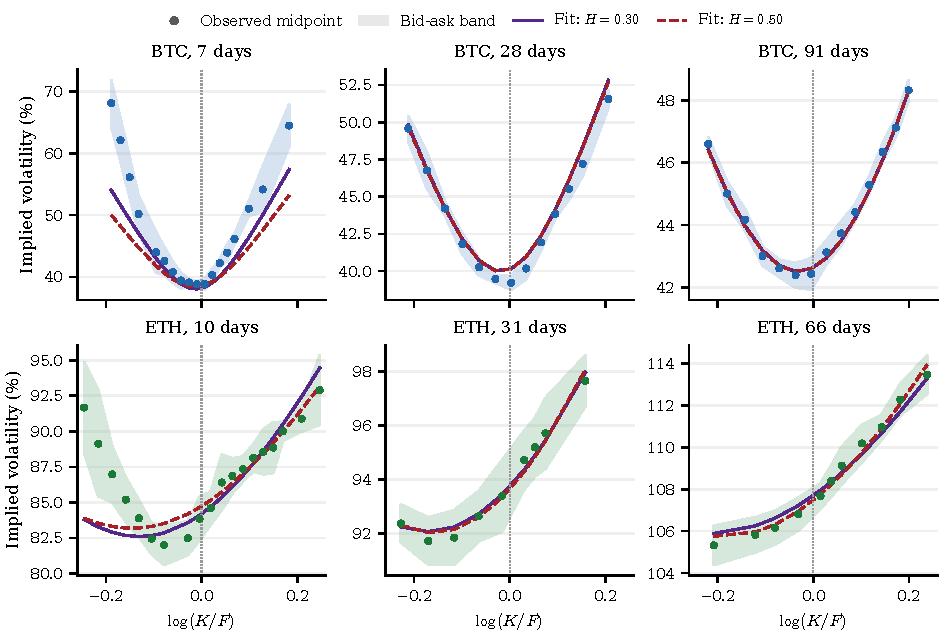
\includegraphics[width=\textwidth]{F1_positive_skew_calibration_final_2026-11-18.pdf}
\caption{Observed Bitcoin and Ether implied-volatility smiles, with bid--ask bands and model fits for both assets at $H=0.30$ (purple, solid) and $H=0.50$ (red, dashed). Bitcoin is observed on 30 June 2023 at 08:00 UTC with maturities 7, 28 and 91 days, and Ether on 26 October 2021 at 08:00 UTC with maturities 10, 31 and 66 days. The 84 retained out-of-the-money Deribit quotes use one common forward per expiry and unchanged coin premiums inverted through $p=\mathrm{Black}(F,K,T,\mathrm{IV})/F$ with unit discounting. Lines connect model values at quoted strikes. Parameters and fit diagnostics are in Table~\ref{tab:calibration}. The cases were selected retrospectively. Data: Deribit quotes archived on 25 October 2026.}\label{fig:motivation}
\end{figure}

% [REVISED 2026-11-23 length: the figure of the stability threshold is removed, its values are in Table tab:critical]

\begin{figure}
\centering
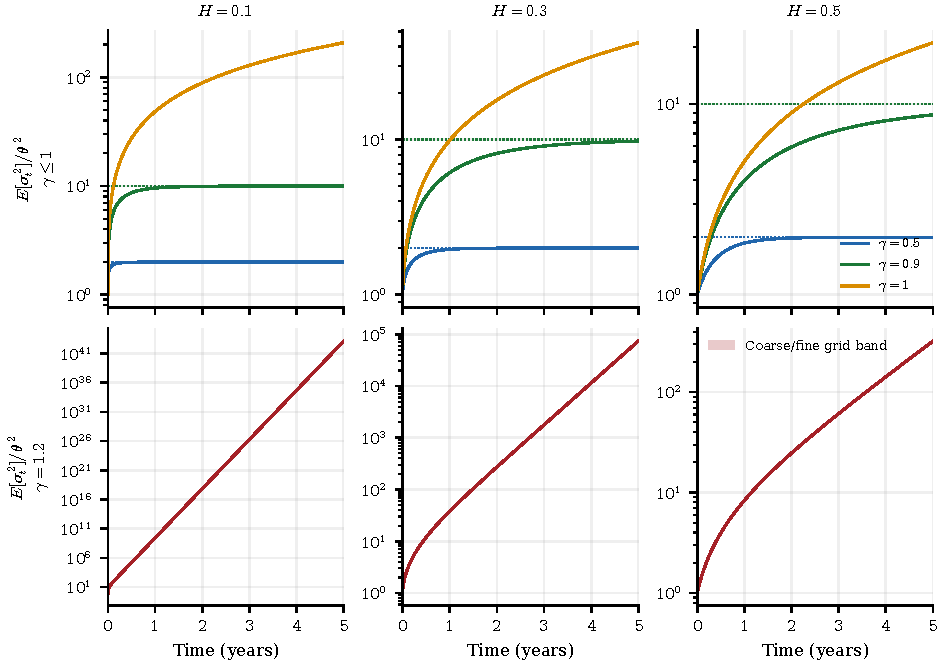
\includegraphics[width=\textwidth]{F3_second_moment_curves.pdf}
\caption{Linear-drift second moments $\E[\sigma_t^2]/\theta^2$ for $\sigma_0=\theta$, $\kappa_1=2$, $\kappa_2=0$ and $H\in\{0.1,0.3,0.5\}$. The top row has $\gamma\in\{0.5,0.9,1\}$, with limits $1/(1-\gamma)$ marked when $\gamma<1$. The bottom row shows $\gamma=1.2$ on separate logarithmic axes. Finite-horizon moments remain finite for every $\gamma$, and the threshold concerns divergence as $t\to\infty$. Shading spans the product-integration solutions on 4,000 and 8,000 steps per year.}\label{fig:moments}
\end{figure}

\begin{figure}
\centering
% [REVISED 2026-11-23 scheme unification] One file for both panels, written by case R2 of ../replication/rough_logsv_scheme_unification.py
% from F4_quadratic_drift_history_R2.json (panel a) and F4_right_panel_time_averaged_history.json (panel b).
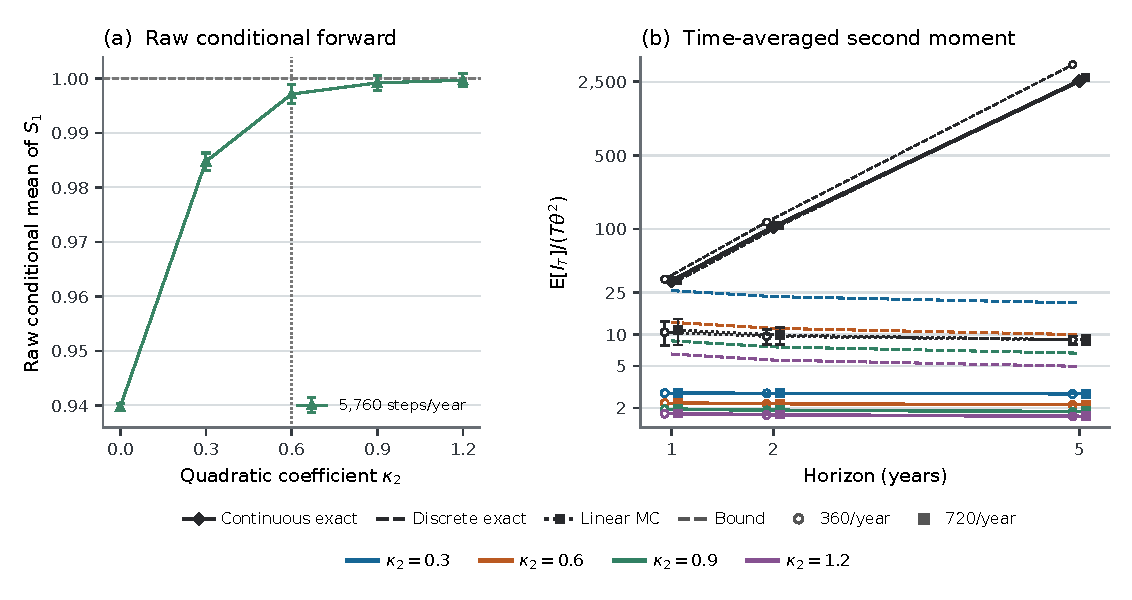
\includegraphics[width=\textwidth]{F4_time_averaged_history_R2.pdf}
\caption{Quadratic-drift diagnostics for the three-factor kernel at $H=0.1$, from the scheme of Appendix~\ref{app:simulation}. Panel (a) shows the sample means of the raw conditional forward of Table~\ref{tab:martingale} at 5,760 steps per year with one per-path standard error. The lines mark a unit forward and $\kappa_2=\beta$. Panel (b) shows the time-averaged second moment $\E[I_T]/(T\theta^2)$ at $T=1,2,5$ years on a logarithmic scale, for $\sigma_0=\theta=0.4$, $\kappa_1=2$, $\rho=0$ and $\vartheta=1.2$ ($\gamma_N=1.0433$). Diamonds give the exact linear-drift values in continuous time. The black dashed lines give the exact linear-drift expectations of the scheme at 360 and 720 steps per year. The coloured dashed lines give the bounds \eqref{eq:cesaro} of Proposition~\ref{prop:cesaro}, which hold for every $\vartheta$. Solid lines give the Monte Carlo estimates for $\kappa_2>0$, and the dotted line gives the Monte Carlo estimates for $\kappa_2=0$ as a control. Open circles and filled squares denote 360 and 720 steps per year, horizontally offset, with one standard error from 40 batch means. Each simulated cell uses 200{,}000 paths from seed 3.}\label{fig:martingale}
\end{figure}

% [GENERATED 2026-11-17 rewritten after the rerun W3 (../agents/sol_results_rough_logsv_W3_2026-11-17.md). Numbers: ../replication/results/F4_right_panel_time_averaged.json, bounds from ../replication/rough_logsv_growth_rate.py.]
% [REVISED 2026-11-23 scheme unification: the Monte Carlo numbers of paragraphs two and three are those of the unified
%  scheme, ../replication/results/F4_right_panel_time_averaged_history.json]
% [REVISED 2026-11-23 length: one paragraph replaces the three paragraphs on panel (b). Numbers as before.]
Panel (b) of Figure~\ref{fig:martingale} fixes the three nodes and weights and takes $\vartheta=1.2$, above the critical value $1.17$ of the linear three-factor model. The exact time-averaged second moment of the linear model, $\E[I_T]/(T\theta^2)$, grows from $32$ at one year to $2{,}540$ at five years. With quadratic drift, Proposition~\ref{prop:cesaro} bounds the same average at five years by $19.9$ for $\kappa_2=0.3$ and by $5.0$ for $\kappa_2=1.2$. The Monte Carlo estimates lie below the bounds in all 24 cells. The Monte Carlo control for $\kappa_2=0$ gives $8.9$ at five years, which is $286$ times below the exact value. For $\kappa_2=0$ the largest $0.1\%$ of the paths carry $40\%$ to $62\%$ of the sample averages, which indicates that the exact moment is carried by paths rarer than the sample contains. A simulated moment that stays flat is therefore not evidence of a bounded moment.
% [END GENERATED 2026-11-17]

% [END REVISED 2026-10-30]

\clearpage
\section{Conclusions and open problems}\label{sec:conclusion}

% [GENERATED 2026-11-17 conclusions restated for the results R1-R4]
We extended log-normal stochastic volatility with quadratic drift to a fractional Volterra equation and proved that it has a unique global non-negative solution with finite moments (Theorem~\ref{thm:wellposed}). For linear drift, exact conditional moments give expected integrated variance and conditional squared VIX. Uniform second-moment boundedness is equivalent to $\gamma<1$, with limiting value $\theta^2/(1-\gamma)$, and above the threshold the second moment grows at the rate $\lambda^*$ of Proposition~\ref{prop:growth}. The explicit constant in \eqref{eq:gamma} makes the threshold reproducible. With a positive quadratic coefficient, the long-run expected integrated variance per unit time is at most $\theta\max(\theta,\kappa_1/\kappa_2)$ for every $\vartheta$ and every $H$ (Proposition~\ref{prop:cesaro}). For the constant kernel the second moment is uniformly bounded (Proposition~\ref{prop:classical_qd}). Theorem~\ref{thm:martingale} gives the martingale property of the price for $\kappa_2\ge\beta$. The change of measure preserves the quadratic polynomial drift, and its density is a true martingale when $\kappa_2^{\Q}\ge0$. Admissible mean-reverting parameters require the restrictions in Proposition~\ref{prop:closure}.

% [REVISED 2026-11-17 after the rerun W3. Numbers: ../replication/results/F4_right_panel_time_averaged.json and ../replication/rough_logsv_growth_rate.py.]
% [REVISED 2026-11-23 scheme unification: factor 286 and two sentences on the scheme. Numbers:
%  ../replication/results/F4_right_panel_time_averaged_history.json and F4_quadratic_drift_history_R2.json]
The linear threshold must be evaluated for the kernel used in a simulation. At $H=0.1$ and $\kappa_1=2$ the three-factor kernel of Figure~\ref{fig:martingale} has critical volatility-of-volatility $1.17$, against $0.95$ for the fractional kernel. At $\vartheta=1.2$, above this threshold, 200{,}000 paths understate the exact five-year time-averaged second moment of the linear-drift model by a factor of about $286$. A flat simulated moment is therefore not evidence of stability. The Monte Carlo scheme of Appendix~\ref{app:simulation} keeps the discrete price an exact martingale on every grid. For $\kappa_2=0$ and $\beta=0.6$ the sample mean of 200{,}000 conditional forwards is $0.940$ against this unit expectation and still decreases at 5,760 steps per year (Table~\ref{tab:martingale}). The marked order-flow construction identifies the candidate drift and covariance, and Proposition~\ref{prop:markov} establishes a stopped constant-kernel limit. The singular-kernel construction is an open problem with additional jump and tightness requirements.

Several analytic questions remain. Strict positivity of the volatility is open for singular kernels (Conjecture~\ref{conj:wellposed}). A pointwise long-horizon second-moment bound and a stationary law under quadratic drift are open for $H<1/2$. The converse martingale statement for $\beta>\kappa_2$ follows from \citet{GuyonJeanninJourdain2026} when $\kappa_2=0$ and the kernel is $K^N$. For $0<\kappa_2<\beta$ and for the fractional kernel it is Conjecture~\ref{conj:supermartingale}. For the order-flow limit, Remark~\ref{conj:limit} explains why limit well-posedness alone is insufficient: vanishing jumps, uniform kernel regularity, boundary control and compact containment also have to be established.
% [GENERATED 2026-11-23 authors' TODO item T7: VIX options under quadratic drift] next two sentences
Proposition~\ref{prop:vix} gives the conditional squared VIX for linear drift only. We leave the valuation of VIX futures and options and the calibration to VIX options in the general case $\kappa_2>0$ for future research.
The selected Bitcoin and Ether calibrations at fixed $H=0.30$ and $H=1/2$ show that positive implied-volatility skew is compatible with positive risk-neutral correlation and the sufficient martingale condition $\kappa_2\ge\beta$.




% [QF 2026-10-31] unnumbered sections required or offered by the journal style; placeholders for the authors.
\section*{Acknowledgements}
\todo{Acknowledgements, if any.}

\section*{Disclosure statement}
\todo{Confirm the journal's standard wording, e.g. ``No potential conflict of interest was reported by the authors.''}

\section*{Data and code availability}
\todo{Confirm: the implementation is in the open-source package StochVolModels (\url{https://github.com/ArturSepp/StochVolModels}); replication scripts and the sealed Deribit snapshot of 25 October 2026 are in the companion \texttt{replication/} folder.}

\bibliographystyle{rQUF}
\bibliography{rough_volterra_lognormal_sv_qf}

\appendices

\section{Proofs}\label{app:proofs}

% [GENERATED 2026-10-08]
\begin{proof}[Proof of Lemma~\ref{lem:factors}] Write $\D Z_s=(\kappa_1+\kappa_2\sigma^N_s)(\theta-\sigma^N_s)\,\D s+\vartheta\sigma^N_s\,\D W^\sigma_s$ and $U^{i}_t=\int_0^te^{-x_i(t-s)}\D Z_s$. Then $\sigma^N_t=\sigma_0+\int_0^tK^N(t-s)\,\D Z_s=\sigma_0+\sum_iw_iU^i_t$, and It\^o's formula gives $\D U^i_t=-x_iU^i_t\,\D t+\D Z_t$. The processes $\sigma^{(i)}=\sigma_{0,i}+U^i$ solve \eqref{eq:factors}, and $\sum_iw_i\sigma^{(i)}=\sigma_0+\sum_iw_iU^i=\sigma^N$. For $s\ge t$, $\int_0^te^{-x_i(s-r)}\D Z_r=e^{-x_i(s-t)}U^i_t$, which gives \eqref{eq:theta_N}.
\end{proof}

% [GENERATED 2026-11-17 proof of global well-posedness with quadratic drift (R1)]
\begin{proof}[Proof of Theorem~\ref{thm:wellposed}] Write $b(x)=c_0+c_1x-dx^2$, and for $n\ge1$ define the truncated drift
\begin{equation*}
b_n(x)=b\big(\min\{\max\{x,-n\},n\}\big).
\end{equation*}
Both kernels satisfy the regularity condition (2.5) of \citet{AbiJaberLarssonPulido2019}. The fractional kernel satisfies it with exponent $2H$ by their Example~2.3(ii), and $K^N$ satisfies it with exponent one because it is bounded and Lipschitz. Both kernels are completely monotone and therefore satisfy their condition (3.4) by their Example~3.7. Constants $C$ below depend on $p$, $T$, $K$ and the coefficients, and they do not depend on $n$.

\emph{Step 1: truncation and non-negativity.} The function $b_n$ is bounded and Lipschitz, and $x\mapsto\vartheta x$ is Lipschitz. Theorem~3.3 of \citet{AbiJaberLarssonPulido2019} gives a unique continuous strong solution $\sigma^n$ of \eqref{eq:sve_general} with $b_n$ in place of the drift $b$. The coefficients are continuous with linear growth, $b_n(0)=c_0\ge0$, and the diffusion coefficient vanishes at zero. Their Theorem~3.6 therefore gives a non-negative continuous weak solution, and pathwise uniqueness identifies its law with the law of $\sigma^n$. Thus $\sigma^n_t\ge0$ for all $t$, almost surely.

\emph{Step 2: one-sided bound.} For $x\ge0$ we have $b_n(x)\le c_0+c_1^+x$, where $c_1^+=\max(c_1,0)$. Since $K\ge0$ and $\sigma^n\ge0$,
\begin{equation}\label{eq:one_sided}
0\le\sigma^n_t\le\sigma_0+c_0\int_0^tK(u)\,\D u+c_1^+\int_0^tK(t-s)\sigma^n_s\,\D s+N^n_t,\qquad N^n_t=\vartheta\int_0^tK(t-s)\sigma^n_s\,\D B_s .
\end{equation}
The quadratic term has dropped out of the upper bound.

\emph{Step 3: moments uniform in $n$.} Fix $p\ge2$ and $T>0$, and let $f_n(t)=\E[(\sigma^n_t)^p]$, which is bounded on $[0,T]$ by Lemma~3.1 of \citet{AbiJaberLarssonPulido2019}. Jensen's inequality gives $\big(\int_0^tK(t-s)\sigma^n_s\,\D s\big)^p\le\big(\int_0^TK(u)\,\D u\big)^{p-1}\int_0^tK(t-s)(\sigma^n_s)^p\,\D s$. For fixed $t$, $N^n_t$ is the terminal value of the martingale $u\mapsto\vartheta\int_0^uK(t-s)\sigma^n_s\,\D B_s$ on $[0,t]$. The Burkholder--Davis--Gundy and Jensen inequalities give $\E|N^n_t|^p\le C\int_0^tK(t-s)^2f_n(s)\,\D s$. Taking the $p$-th power and expectations in \eqref{eq:one_sided} yields
\begin{equation*}
f_n(t)\le C+C\int_0^t\big(K(t-s)+K(t-s)^2\big)f_n(s)\,\D s,\qquad t\le T .
\end{equation*}
Choose $\varrho>0$ with $C\int_0^Te^{-\varrho u}\big(K(u)+K(u)^2\big)\D u\le1/2$, which is possible because $K+K^2$ is integrable on $[0,T]$. Multiplying the inequality by $e^{-\varrho t}$ and taking the supremum over $t\le T$ gives $\sup_{t\le T}e^{-\varrho t}f_n(t)\le2C$, so that $\sup_n\sup_{t\le T}f_n(t)\le2Ce^{\varrho T}$.

\emph{Step 4: supremum bound.} On $x\ge0$, $|b_n(x)|\le c_0+|c_1|x+dx^2$, so Step~3 with $2p$ in place of $p$ bounds $\sup_{t\le T}\E|b_n(\sigma^n_t)|^p$ uniformly in $n$. Lemma~2.4 of \citet{AbiJaberLarssonPulido2019} then gives $\E\big[\sup_{t\le T}(\sigma^n_t)^p\big]\le C$ for $p>\max\{2,1/H\}$, and for $p>2$ in the case of $K^N$. With $\tau_n=\inf\{t\ge0:\sigma^n_t\ge n\}$, Markov's inequality gives
\begin{equation}\label{eq:tau_n}
\P(\tau_n\le T)\le Cn^{-p} .
\end{equation}

\emph{Step 5: local uniqueness and removal of the truncation.} Let $X$ and $Y$ be continuous adapted processes and let $\tau$ be the first time that $|X|$ or $|Y|$ reaches $n$. Assume that, up to $\tau$, both satisfy \eqref{eq:sve_general} with the same Brownian motion and with drifts that coincide with $b$ on $[-n,n]$. On $\{t\le\tau\}$ both drift integrands equal $b$ evaluated in $[-n,n]$, where $b$ is Lipschitz, and the indicator $\one_{\{s\le\tau\}}$ can be inserted in both integrals. The function $\Delta(t)=\E\big[|X_t-Y_t|^2\one_{\{t\le\tau\}}\big]$ therefore satisfies $\Delta(t)\le C_n\int_0^t\big(K(t-s)+K(t-s)^2\big)\Delta(s)\,\D s$, and the argument of Step~3 gives $\Delta\equiv0$, that is, $X=Y$ on $[0,\tau]$. In particular $\sigma^m=\sigma^n$ on $[0,\tau_n]$ for $m\ge n$, the times $\tau_n$ increase, and $\tau_n\to\infty$ almost surely by \eqref{eq:tau_n}. The limit $\sigma=\lim_n\sigma^n$ is continuous and non-negative. The limit solves \eqref{eq:sve_general} on $[0,\infty)$, because $b_n(\sigma^n)=b(\sigma)$ on $[0,\tau_n]$ and stochastic integrals of integrands that agree on an event agree on that event. The same local argument gives pathwise uniqueness among continuous solutions. The moment bound follows from Step~4 and Fatou's lemma, first for large $p$ and then for every $p\ge1$ by Jensen's inequality.
\end{proof}
% [END GENERATED 2026-11-17]

% [REVISED 2026-10-30 a priori moment bound replaces the forward reference to Proposition second]
\begin{proof}[Proof of Proposition~\ref{prop:mean}] For $\kappa_2=0$ the coefficients are globally Lipschitz with linear growth. Lemma~3.1 of \citet{AbiJaberLarssonPulido2019} gives $\sup_{s\le T}\E[\sigma_s^2]<\infty$ on every finite horizon, and their Example~2.3(ii) verifies the kernel regularity. The stochastic integral in \eqref{eq:flow} is square integrable since $K\in L^2_{\rm loc}$, and has zero conditional mean. Therefore $m_t(s)=\Theta^t_s+\kappa_1\int_t^sK(s-r)(\theta-m_t(r))\,\D r$. Writing $\phi=m_t-\theta$ gives $\phi=\psi_t-\kappa_1K*\phi$ on $[t,\infty)$, so \eqref{eq:resolvent} yields $\phi=\psi_t-R*\psi_t$. At $t=0$, $\psi_0\equiv\sigma_0-\theta$, giving the unconditional mean. For the fractional kernel, $\widehat R(z)=\kappa_1/(z^\alpha+\kappa_1)$, which inverts to \eqref{eq:resolvent_frac}. When $\kappa_1=0$, $R=0$.
\end{proof}

\begin{proof}[Proof of Proposition~\ref{prop:second}] Subtracting the equation for $m_t$ from \eqref{eq:flow}, the centred process $\chi_s=\sigma_s-m_t(s)$ solves $\chi=-\kappa_1K*\chi+K*\D M$ on $[t,\infty)$, with $\D M_r=\vartheta\sigma_r\,\D W^\sigma_r$. The process $G*\D M$ solves the same linear equation, because $G=K-\kappa_1K*G$, by \eqref{eq:resolvent} when $\kappa_1>0$ and directly from $G=K$ when $\kappa_1=0$, together with the stochastic Fubini theorem. Uniqueness for the linear equation gives $\chi_s=\int_t^sG(s-r)\vartheta\sigma_r\,\D W^\sigma_r$. It\^o's isometry yields $\E[\chi_s^2\mid\F_t]=\vartheta^2\int_t^sG(s-r)^2v_t(r)\,\D r$, and $v_t(s)=m_t(s)^2+\E[\chi_s^2\mid\F_t]$ because $\E[\chi_s\mid\F_t]=0$. The a priori bound in the proof of Proposition~\ref{prop:mean} makes every term finite.
\end{proof}

\begin{proof}[Proof of Corollary~\ref{cor:ml}] With $\kappa_1=0$, $G=K$ and $m\equiv\sigma_0$. Since $\vartheta^2K(t)^2=a\,t^{2H-1}/\Gamma(2H)$, equation \eqref{eq:cond_second} at $t=0$ reads $v=\sigma_0^2+a\,\mathcal{I}^{2H}v$, where $\mathcal{I}^{2H}$ is the Riemann--Liouville integral of order $2H$. Its solution is $\sigma_0^2E_{2H}(a\,t^{2H})$, and integration term by term gives $\E[I_T]$. The asymptotics follow from $E_{2H}(z)\sim(2H)^{-1}\exp(z^{1/(2H)})$ as $z\to+\infty$ \citep{GorenfloKilbasMainardiRogosin2014}.
\end{proof}

\begin{proof}[Proof of Proposition~\ref{prop:vix}] For continuous paths, $-\tfrac2\Delta\E[\ln(S_{T+\Delta}/S_T)\mid\F_T]=\tfrac1\Delta\E[I_{T+\Delta}-I_T\mid\F_T]=\tfrac1\Delta\int_T^{T+\Delta}v_T(s)\,\D s$. Substituting $v_T=m_T^2+\widetilde R*m_T^2$ from Proposition~\ref{prop:second} and exchanging the order of integration gives \eqref{eq:vix}. Under $K^N$, \eqref{eq:theta_N} makes $\psi_T$ affine in $u$, and \eqref{eq:cond_mean} preserves affinity. The square $m_T^2$ is then a quadratic form in $u$, and so is its integral against $\varpi_T$.
\end{proof}

% [REVISED 2026-11-17 localisation proof completed with Theorem wellposed (R2); proof of the density corollary added]
\begin{proof}[Proof of Theorem~\ref{thm:martingale}]
The stochastic exponential $S/S_0$ is a positive local martingale and hence a supermartingale. By Theorem~\ref{thm:wellposed} the volatility is non-negative and does not explode. For $n>\sigma_0$, define $\tau_n=\inf\{t\ge0:\sigma_t\ge n\}$, with $\inf\varnothing=\infty$. The stopped price is a martingale by Novikov's criterion, because $\int_0^{T\wedge\tau_n}\sigma_s^2\D s\le n^2T$. Define
\begin{equation*}
\left.\frac{\D\widehat\Q^{(n)}}{\D\Q}\right|_{\F_T}=\frac{S_{T\wedge\tau_n}}{S_0}.
\end{equation*}
Then $\widehat W^{(0,n)}_t=W^{(0)}_t-\int_0^{t\wedge\tau_n}\sigma_u\D u$ and $W^{(1)}$ form a two-dimensional Brownian motion under $\widehat\Q^{(n)}$, and $\widehat B=(\beta\widehat W^{(0,n)}+\varepsilon W^{(1)})/\vartheta$ is a Brownian motion. Up to $\tau_n$, the volatility satisfies \eqref{eq:sve_general} with respect to $\widehat B$, with drift
\begin{equation*}
(\kappa_1+\kappa_2\sigma)(\theta-\sigma)+\beta\sigma^2
=\kappa_1\theta-(\kappa_1-\kappa_2\theta)\sigma-(\kappa_2-\beta)\sigma^2.
\end{equation*}
Let $\widehat\sigma$ be the global solution of \eqref{eq:sve_general} driven by $\widehat B$ with $c_0=\kappa_1\theta$, $c_1=\kappa_2\theta-\kappa_1$ and $d=\kappa_2-\beta\ge0$, which exists by Theorem~\ref{thm:wellposed}. Let $\widehat\tau_n$ be the first time that $\widehat\sigma$ reaches $n$. Step~5 of the proof of Theorem~\ref{thm:wellposed} gives $\sigma=\widehat\sigma$ on $[0,\tau_n\wedge\widehat\tau_n]$, and therefore $\tau_n=\widehat\tau_n$. The law of $\widehat\sigma$ does not depend on $n$, so the moment bound of Theorem~\ref{thm:wellposed} and Markov's inequality give $\widehat\Q^{(n)}(\tau_n\le T)\le Cn^{-p}$ with $C$ independent of $n$. Thus
\begin{equation*}
\frac{\E_{\Q}[S_T\one_{\{\tau_n>T\}}]}{S_0}
=\widehat\Q^{(n)}(\tau_n>T)
\ge1-Cn^{-p}\longrightarrow1.
\end{equation*}
Since $\one_{\{\tau_n>T\}}\uparrow1$ almost surely, monotone convergence yields $\E_{\Q}[S_T]=S_0$. A non-negative supermartingale whose expectation is unchanged over $[0,T]$ is a martingale, proving the claim.
\end{proof}

\begin{proof}[Proof of Corollary~\ref{cor:density}] Denote the stochastic exponential in \eqref{eq:density} by $D$. The process $D$ is a positive $\P$-local martingale, and with $\tau_n$ as in the previous proof the stopped process $D_{\cdot\wedge\tau_n}$ is a martingale by Novikov's criterion. Under the measure with density $D_{T\wedge\tau_n}$, the substitution that proves Proposition~\ref{prop:closure} shows that, up to $\tau_n$, the volatility satisfies \eqref{eq:sve_general} with $c_0=\kappa_1\theta$, $c_1=\kappa_2\theta-\kappa_1$ and $d=\kappa_2^{\Q}$. For $\kappa_2^{\Q}\ge0$ the argument of the previous proof gives $\E_{\P}[D_T\one_{\{\tau_n>T\}}]\ge1-Cn^{-p}$, and therefore $\E_{\P}[D_T]=1$.
\end{proof}
% [END REVISED 2026-11-17]


% [GENERATED 2026-10-24]
\begin{proof}[Proof of Proposition~\ref{prop:stationarity}] The mean $m(t)=\theta+(\sigma_0-\theta)E_\alpha(-\kappa_1t^\alpha)$ lies between $\sigma_0$ and $\theta$, so $m^2$ is bounded above and below by a positive constant, and $m^2\to\theta^2$. The kernel $h=\vartheta^2G^2$ is non-negative and integrable: $G(t)\sim t^{\alpha-1}/\Gamma(\alpha)$ at zero with $\alpha>1/2$, and $G$ decays as $O(t^{-1-\alpha})$ for $\alpha<1$ and exponentially at $\alpha=1$. Its positive resolvent has the locally convergent convolution series $\widetilde R=\sum_{j\ge1}h^{*j}$. Tonelli's theorem gives
\begin{equation*}
\int_0^\infty\widetilde R(s)\,\D s
=\sum_{j\ge1}\Big(\int_0^\infty h(s)\,\D s\Big)^j
=\sum_{j\ge1}\gamma^j.
\end{equation*}
If $\gamma<1$, Proposition~\ref{prop:second} gives $\sup v\le\sup m^2/(1-\gamma)$, and dominated convergence in $\widetilde R*m^2$ gives $v(t)\to\theta^2/(1-\gamma)$. If $\gamma\ge1$, then with $\underline m=\min(\sigma_0,\theta)>0$,
$v(t)\ge\underline m^2(1+\int_0^t\widetilde R(s)\,\D s)\to\infty$.
% [GENERATED 2026-11-17] next sentence
This direction needs only $\theta\ne0$. If $m(s)^2\ge\theta^2/4$ for $s\ge s_0$, then $v(t)\ge(\theta^2/4)\int_0^{t-s_0}\widetilde R(s)\,\D s\to\infty$.
For the norm, $\widehat G(z)=1/(z^\alpha+\kappa_1)$ and Parseval's identity imply
\begin{equation*}
\int_0^\infty G^2=\frac1{2\pi}\int_{-\infty}^\infty
\frac{\D\omega}{|\omega|^{2\alpha}+2\kappa_1|\omega|^\alpha\cos(\pi\alpha/2)+\kappa_1^2}.
\end{equation*}
The substitution $\omega=\kappa_1^{1/\alpha}u$ gives the factor $\kappa_1^{1/\alpha-2}$. For $\alpha<1$, substituting $y=u^\alpha$ in the remaining integral and integrating the two complex-conjugate linear factors gives
\begin{equation*}
C(\alpha)=-\frac{\cot(\pi\alpha/2)}{\alpha\sin(\pi/\alpha)}.
\end{equation*}
At $\alpha=1$, direct integration gives $C(1)=1/2$, also the limit of this expression.
\end{proof}

% [GENERATED 2026-11-17 proof of the growth rate (R4)]
\begin{proof}[Proof of Proposition~\ref{prop:growth}] Parseval's identity gives the second expression in \eqref{eq:h_hat}. We apply it to $u\mapsto e^{-\lambda u/2}G(u)$, whose Laplace transform on the imaginary axis is
\begin{equation*}
\widehat G(\lambda/2+\mathrm{i}\omega)=\big((\lambda/2+\mathrm{i}\omega)^\alpha+\kappa_1\big)^{-1}.
\end{equation*}
The function $\widehat h$ is continuous and strictly decreasing, and $\widehat h(0+)=\gamma$ by monotone convergence. For $\kappa_1>0$, dominated convergence gives $\widehat h(\lambda)\to0$ as $\lambda\to\infty$, and for $\kappa_1=0$ the transform is $a\lambda^{-2H}$ with $a$ from \eqref{eq:ml_second}. For $\gamma>1$ the root $\lambda^*$ therefore exists and is unique. Equation \eqref{eq:cond_second} at $t=0$ reads $v=m^2+h*v$. Multiplying by $e^{-\lambda^*t}$ gives the renewal equation $v^*=z+h^**v^*$ for $v^*(t)=e^{-\lambda^*t}v(t)$, with $z(t)=e^{-\lambda^*t}m(t)^2$ and $h^*(t)=e^{-\lambda^*t}h(t)$. The function $h^*$ is a probability density with finite mean $\int_0^\infty u\,h^*(u)\,\D u=|\widehat h'(\lambda^*)|$. The function $z$ is continuous and bounded by a multiple of $e^{-\lambda^*t}$, and is therefore directly Riemann integrable. The key renewal theorem \citep[Chapter~XI]{Feller1971} gives $v^*(t)\to|\widehat h'(\lambda^*)|^{-1}\int_0^\infty z(s)\,\D s$, which is \eqref{eq:growth}. For $\sigma_0=\theta$ we have $m\equiv\theta$ and $\int_0^\infty z(s)\,\D s=\theta^2/\lambda^*$.

For $\gamma=1$ the kernel $h$ itself is a probability density. Its mean $\mu_h$ is finite, because $u\,G(u)^2$ is of order $u^{2\alpha-1}$ at zero and of order $u^{-1-2\alpha}$ at infinity for $\alpha<1$, and decays exponentially at $\alpha=1$. The solution is $v=m^2+\widetilde R*m^2$, where $\widetilde R=\sum_{j\ge1}h^{*j}$ is the renewal density. The renewal theorem gives $t^{-1}\int_0^t\widetilde R(s)\,\D s\to1/\mu_h$. Since $m^2$ is bounded and $m^2\to\theta^2$, splitting the convolution at a fixed distance from $t$ gives $v(t)/t\to\theta^2/\mu_h$.
\end{proof}
% [END GENERATED 2026-11-17]

\begin{proof}[Proof of Proposition~\ref{prop:markov}] For $K\equiv1$, set $\delta=\vartheta/\sqrt n$. The Markov chain $(\sigma^n,P^n)$ has jumps $(\delta\zeta,n^{-1/2}\eta)$ at rate $n\sigma^2$, where $\zeta$ and $\eta$ denote the marks of a trade. For $f\in C_c^\infty((0,\infty)\times\mathbb R)$ its generator is $A_nf(\sigma,p)=n\sigma^2\,\E\big[f(\sigma+\delta\zeta,p+n^{-1/2}\eta)-f(\sigma,p)\big]$. Taylor expansion and the mark moments in \eqref{eq:bias} give
\begin{equation*}
A_nf=\sqrt n\,\vartheta\sigma^2\beta_n\,\partial_\sigma f+\tfrac12\vartheta^2\sigma^2\,\partial_{\sigma\sigma}f+\tfrac12\sigma^2\,\partial_{pp}f+\rho(1-|\beta_n|)\vartheta\sigma^2\,\partial_{\sigma p}f+O(n^{-1/2}),
\end{equation*}
uniformly on compact subsets of $(0,\infty)\times\mathbb R$. Fix the domain $D$ of the proposition. On a neighbourhood of its closure the clip is inactive for all sufficiently large $n$, so the first coefficient equals $(\kappa_1+\kappa_2\sigma)(\theta-\sigma)$ and $|\beta_n|\to0$ uniformly. Thus $A_n$ converges there to the generator of \eqref{eq:markov_limit}. The stopped drift and predictable quadratic-variation rates are uniformly bounded, and the jump sizes tend to zero. These bounds give tightness of the stopped martingale problems, and every limit has continuous paths. The limiting coefficients are locally Lipschitz. On $\overline D$ the covariance matrix is uniformly positive definite because $\sigma\ge\sigma_->0$ and $1-\rho^2=\varepsilon^2/\vartheta^2>0$. Therefore the stopped diffusion law is unique, and the boundary of the rectangle is regular for exit. Localisation of the diffusion-approximation argument of \citet{EthierKurtz1986} identifies the limit as the diffusion stopped on leaving $D$, and the chain's exit overshoot tends to zero with its jump size. These steps prove the stated stopped convergence. Removing the stops requires uniform exit estimates for the chains as $\sigma_-\downarrow0$ and $\sigma_+,R\uparrow\infty$, which are not supplied here.
\end{proof}

% [REVISED 2026-10-30 proof moved here from the proof of Proposition markov (C7)]
\begin{proof}[Proof of Proposition~\ref{prop:classical_qd}] For $K\equiv1$ the volatility is the diffusion $\D\sigma=b(\sigma)\,\D t+\vartheta\sigma\,\D W^\sigma$ on $(0,\infty)$, where $b(\sigma)=\kappa_1\theta-(\kappa_1-\kappa_2\theta)\sigma-\kappa_2\sigma^2$. Its speed density is proportional to
\begin{equation*}
\sigma^{-2}\exp\left(\int \frac{2b(\sigma)}{\vartheta^2\sigma^2}\,\D\sigma\right),
\end{equation*}
which gives \eqref{eq:stationary_density}. Put $A=2\kappa_1\theta/\vartheta^2>0$, $B=2\kappa_2/\vartheta^2>0$ and $c=2(\kappa_1-\kappa_2\theta)/\vartheta^2$. The scale and speed densities are proportional to $\sigma^c e^{A/\sigma+B\sigma}$ and $\sigma^{-c-2}e^{-A/\sigma-B\sigma}$. The scale integrals diverge at both endpoints, excluding access from the interior, while the entrance integrals are finite, so both endpoints are entrance boundaries. The finite speed measure normalises to the stationary law. The factors $e^{-B\sigma}$ and $e^{-A/\sigma}$ make all positive and negative stationary moments finite.
For a deterministic initial state, the generator satisfies
\begin{equation*}
\mathcal L\sigma^2=2\kappa_1\theta\sigma+
(-2\kappa_1+2\kappa_2\theta+\vartheta^2)\sigma^2-2\kappa_2\sigma^3
\le C-c_2\sigma^2
\end{equation*}
for some $C,c_2>0$. The stopped It\^o estimate and localisation therefore give
$\E[\sigma_t^2]\le e^{-c_2t}\sigma_0^2+C(1-e^{-c_2t})/c_2$, proving uniform boundedness.
\end{proof}

% [GENERATED 2026-11-17 proof of the time-averaged bound (R3), restated for both kernels in the amendment of r2]
\begin{proof}[Proof of Proposition~\ref{prop:cesaro}] Let $b(x)=\kappa_1\theta+c_1x-\kappa_2x^2$ with $c_1=\kappa_2\theta-\kappa_1$, and define the semimartingale $Z_t=\int_0^tb(\sigma_s)\,\D s+\vartheta\int_0^t\sigma_s\,\D W^\sigma_s$, so that $\sigma-\sigma_0=K*\D Z$. Both kernels are completely monotone. By Example~3.7 of \citet{AbiJaberLarssonPulido2019} they satisfy their condition (3.4), which includes a non-negative resolvent of the first kind $L$. For the fractional kernel with $\alpha<1$, $L(\D s)=s^{-\alpha}\,\D s/\Gamma(1-\alpha)$ and $L([0,T])=T^{1-\alpha}/\Gamma(2-\alpha)$. At $\alpha=1$, $L=\delta_0$ and $L([0,T])=1$, which is the same expression. Their Lemma~2.6 gives $Z=L*(\sigma-\sigma_0)$. Since $\sigma\ge0$ by Theorem~\ref{thm:wellposed} and $L\ge0$,
\begin{equation}\label{eq:Z_lower}
Z_T=\int_{[0,T]}(\sigma_{T-s}-\sigma_0)\,L(\D s)\ge-\sigma_0\,L([0,T]) .
\end{equation}
The moments of Theorem~\ref{thm:wellposed} make the stochastic integral in $Z$ a martingale. With $m(t)=\E[\sigma_t]$ and $v(t)=\E[\sigma_t^2]$, taking expectations in \eqref{eq:Z_lower} gives
\begin{equation*}
\kappa_2\int_0^Tv(t)\,\D t\le\kappa_1\theta\,T+c_1\int_0^Tm(t)\,\D t+\sigma_0\,L([0,T]) .
\end{equation*}
If $c_1\le0$ we drop the middle term, because $m\ge0$. If $c_1>0$ we use $m\le\sqrt v$ and the Cauchy--Schwarz inequality, $\int_0^Tm(t)\,\D t\le\big(T\int_0^Tv(t)\,\D t\big)^{1/2}=T\sqrt{A_T}$. Division by $T$ gives \eqref{eq:cesaro}, which is a quadratic inequality in $\sqrt{A_T}$. Thus $\sqrt{A_T}$ is at most the positive root $y_T$ of $\kappa_2y^2-c_1^+y-\kappa_1\theta-\sigma_0L([0,T])/T=0$, and $y_T$ increases with the last term.

For the fractional kernel the last term tends to zero as $T\to\infty$. If $c_1\le0$, then $y_T^2\to\kappa_1\theta/\kappa_2$, and $\kappa_1/\kappa_2\ge\theta$ in this case. If $c_1>0$, then $y_T\to\big(c_1+\sqrt{c_1^2+4\kappa_2\kappa_1\theta}\big)/(2\kappa_2)=\theta$, because $c_1^2+4\kappa_2\kappa_1\theta=(\kappa_2\theta+\kappa_1)^2$, and $\theta>\kappa_1/\kappa_2$ in this case. Both cases give \eqref{eq:cesaro_limit}.

For $K^N$ put $k(t)=\int_0^tK^N(s)\,\D s$. We integrate $K^N*L\equiv1$ over $[0,T]$ and exchange the order of integration, which gives $T=\int_{[0,T]}k(T-s)\,L(\D s)$ for every $T>0$. The function $k$ is non-decreasing and $L\ge0$, so that $T\le k(T)\,L([0,T])$. The same identity at $T+a$ gives $T+a\ge k(a)\,L([0,T])$ for every $a>0$, because $k(T+a-s)\ge k(a)$ for $s\le T$. Thus
\begin{equation*}
\frac{1}{k(T)}\le\frac{L([0,T])}{T}\le\frac{1+a/T}{k(a)} .
\end{equation*}
We let $T\to\infty$ and then $a\to\infty$ and obtain $L([0,T])/T\to1/k(\infty)=\ell_N$. The limit of $y_T^2$ is the right-hand side of \eqref{eq:cesaro_limit_N}.
\end{proof}
% [END GENERATED 2026-11-17]

\section{Simulation scheme and validation}\label{app:simulation}

% [GENERATED 2026-11-23 scheme unification. This appendix replaces the description of the split-step scheme, whose text of
%  17 November 2026 is kept in ../drafts/r4_pre_unification_2026-11-23/. It describes the scheme of the module
%  stochvolmodels/models/rough_logsv/history.py, which produced Table 5 and now produces Tables 4 and B1 and Figure 4.
%  Formula sheet: ../agents/sol_results_rough_logsv_scheme_unification_2026-11-23.md. The step as written here agrees with an
%  independent replay of the package arithmetic to 2.5e-13 (../agents/implementation_2026-11-23/check_paper_form.py).]
\subsection{Symmetric splitting of the factor system}\label{sec:splitting}

We approximate the factor system \eqref{eq:factors} on a uniform grid $t_n=nh$. In this appendix grid-time state symbols denote the numerical approximation, rather than the exact solution. Every path carries all $N$ factors, so the state at $t_n$ contains the full history of the Markovian model.

Write $c_0=\kappa_1\theta$ and $c_1=\kappa_2\theta-\kappa_1$ as in \eqref{eq:sve_general}. The Stratonovich form of \eqref{eq:factors} is
\begin{equation}\label{eq:factors_strat}
\D\sigma^{(i)}_t=\Big[-x_i\big(\sigma^{(i)}_t-\sigma_{0,i}\big)+c_0+\tilde c_1\sigma^N_t-\kappa_2\big(\sigma^N_t\big)^2\Big]\D t+\vartheta\sigma^N_t\circ\D W^\sigma_t,\qquad \tilde c_1=c_1-\tfrac12\bar w\vartheta^2 .
\end{equation}
The correction $-\tfrac12\bar w\vartheta^2\sigma^N$ is the same for every factor, because every factor receives the noise $\vartheta\sigma^N\D W^\sigma$ and $\sigma^N$ has the derivative $w_j$ with respect to $\sigma^{(j)}$.

We split the right-hand side of \eqref{eq:factors_strat} into a linear part, the quadratic damping and the noise. Each part has a flow in closed form, and the linear part contains the decay rates $x_i$, which are the stiff terms of the system. Let $\boldsymbol U=(U^1,\dots,U^N)^\top$ with $U^i=\sigma^{(i)}-\sigma_{0,i}$ denote the centred factors of the proof of Lemma~\ref{lem:factors}, so that $\sigma^N=\sigma_0+w^\top\boldsymbol U$, and let $\one$ denote the vector of ones. The memory map $\mathcal{M}_\tau$ solves the linear part $\D\sigma^{(i)}/\D t=-x_i(\sigma^{(i)}-\sigma_{0,i})+c_0+\tilde c_1\sigma^N$ over a time $\tau$,
\begin{equation}\label{eq:memory_map}
\mathcal{M}_\tau:\ \boldsymbol U\mapsto\boldsymbol U^\ast+e^{-\Lambda\tau}\big(\boldsymbol U-\boldsymbol U^\ast\big),\qquad \Lambda=\mathrm{diag}(x)-\tilde c_1\one w^\top,\qquad \boldsymbol U^\ast=(c_0+\tilde c_1\sigma_0)\,\Lambda^{-1}\one .
\end{equation}
The damping map $\mathcal{D}_\tau$ solves $\D\sigma^{(i)}/\D t=-\kappa_2(\sigma^N)^2$ over a time $\tau$, and the noise map $\mathcal{N}_h$ solves $\D\sigma^{(i)}=\vartheta\sigma^N\circ\D W^\sigma$ over one step. Both maps act on the weighted sum,
\begin{equation}\label{eq:scalar_maps}
\mathcal{D}_\tau:\ \sigma^N\mapsto\frac{\sigma^N}{1+\bar w\kappa_2\tau\,\sigma^N},\qquad
\mathcal{N}_h:\ \sigma^N\mapsto\sigma^N\exp\big(\bar w\vartheta\sqrt h\,Z^\sigma\big),
\end{equation}
with $Z^\sigma$ standard normal, and both add the same amount to every factor, which is the change of $\sigma^N$ divided by $\bar w$. One step of the scheme is the symmetric composition
\begin{equation}\label{eq:scheme}
\boldsymbol U_{n+1}=\mathcal{M}_{h/2}\circ\mathcal{D}_{h/2}\circ\mathcal{N}_h\circ\mathcal{D}_{h/2}\circ\mathcal{M}_{h/2}\big(\boldsymbol U_n\big),
\end{equation}
with one normal variable $Z^\sigma_n$ per step.

The memory map integrates the decay rates exactly, so the largest node does not restrict the time step. For the kernel of the calibration the largest node is $7.4\times10^6$ per year. Conjugation with $\mathrm{diag}(\sqrt{w_i})$ makes $\Lambda$ symmetric, and the implementation diagonalises the symmetric matrix once for each parameter vector and time step.\footnote{Functions \texttt{prepare\_history} and \texttt{simulate\_history} of the module \path{stochvolmodels/models/rough_logsv/history.py}.} The implementation requires the smallest eigenvalue of $\Lambda$ to be positive, which holds whenever $\tilde c_1<0$ and all nodes are positive. This requirement belongs to the numerical method, and Theorem~\ref{thm:wellposed} does not need it.

The damping and noise maps keep a positive $\sigma^N$ positive. The memory map is affine and does not guarantee a positive $\sigma^N$ for $N>1$. The implementation stops with an error if a volatility state is non-positive or not finite, and uses no floor, no reset of the state and no deletion of paths. All runs behind Tables~\ref{tab:martingale} and~\ref{tab:validation} and Figure~\ref{fig:martingale} completed without such an error.

% [REVISED 2026-11-23 sweep: attribution of the composition of Stratonovich flows]
Each of the three flows is exact, and their composition \eqref{eq:scheme} approximates the solution of \eqref{eq:factors}. \citet{NinomiyaVictoir2008} compose the flows of the Stratonovich vector fields in their weak scheme of second order, and \citet{BayerBreneis2024} use splitting schemes of this type for the Markovian approximation of rough Heston. We do not prove a convergence order for \eqref{eq:scheme}. Section~\ref{sec:validation} measures its time-discretisation error against exact moments.

\subsection{Price step and the discrete martingale}\label{sec:price_step}

The price step holds the volatility at its value $\sigma^N_n$ at the beginning of the step,
\begin{equation}\label{eq:price_step}
\begin{split}
I_{n+1}&=I_n+\big(\sigma^N_n\big)^2h,\qquad J_{n+1}=J_n+\sigma^N_n\sqrt h\,Z^\sigma_n,\\
X_{n+1}&=X_n-\tfrac12\big(\sigma^N_n\big)^2h+\sigma^N_n\sqrt h\,\Big(\rho Z^\sigma_n+\sqrt{1-\rho^2}\,Z^\perp_n\Big),
\end{split}
\end{equation}
with $I_0=J_0=0$. Here $Z^\sigma_n$ is the normal variable of the noise map in step $n$, and $Z^\perp_n$ is a standard normal variable that is independent of all other variables. The sums $I_n$ and $J_n$ are the left-point sums of $\int(\sigma^N_u)^2\,\D u$ and $\int\sigma^N_u\,\D W^\sigma_u$. A left-point sum has a first-order error in $h$, where a symmetric rule would have a second-order error. We accept the first-order error, because the left point is known at the beginning of the step and gives the following property.

\begin{lemma}[Discrete martingale]\label{lem:discrete_martingale}
Suppose that the volatility states $\sigma^N_n$ of the scheme \eqref{eq:scheme} are finite almost surely. Then, for every step $h>0$, every $\kappa_2\ge0$ and every $\rho\in[-1,1]$, the discrete price $S_n=S_0e^{X_n-X_0}$ of \eqref{eq:price_step} is a martingale, and $\E[S_n]=S_0$ for every $n$. The same holds for $S_0\exp\big(\rho J_n-\tfrac12\rho^2I_n\big)$.
\end{lemma}

\begin{proof}[Proof of Lemma~\ref{lem:discrete_martingale}] The state $\sigma^N_n$ is a function of $Z^\sigma_0,\dots,Z^\sigma_{n-1}$. Conditional on the normal variables of the first $n$ steps, the ratio $S_{n+1}/S_n$ is therefore log-normal with unit mean, and the conditional expectation of $S_{n+1}$ is $S_n$. The tower property for non-negative variables gives $\E[S_{n+1}]=\E[S_n]=S_0$, so that $S_n$ is integrable. The second statement follows in the same way, with $\rho Z^\sigma_n$ in place of $\rho Z^\sigma_n+\sqrt{1-\rho^2}\,Z^\perp_n$ and $\rho^2(\sigma^N_n)^2h$ in place of $(\sigma^N_n)^2h$.
\end{proof}

% [GENERATED 2026-11-23 scheme unification] the next paragraph is crux text for the authors' rewrite
Lemma~\ref{lem:discrete_martingale} places no restriction on $\kappa_2$ and $\beta$. For $\kappa_2=0$, $\beta>0$ and the kernel $K^N$ the continuous-time price is a strict local martingale (Section~\ref{sec:measure}), so that $\E[S_T]<S_0$, while $\E[S_n]=S_0$ on every grid. The two statements are compatible, because convergence of the discrete price in distribution does not imply convergence of its expectation. On a fine grid the missing expectation is carried by paths of small probability, and a sample mean below $S_0$ measures the part of the expectation that the sample does not contain. Table~\ref{tab:martingale} reports this deficit and its dependence on the grid.

\subsection{Conditional Monte Carlo and the half-tilted measure}\label{sec:conditional_mc}

Conditional on the volatility normals $Z^\sigma_0,\dots,Z^\sigma_{n-1}$, the log return $L_n=X_n-X_0$ of \eqref{eq:price_step} is Gaussian with mean $\rho J_n-\tfrac12I_n$ and variance $(1-\rho^2)I_n$. With $F=S_0$ under our zero-rate convention, a European payoff has the conditional price of Black's formula with forward and total variance
\begin{equation}\label{eq:conditional_forward}
F_n=F\exp\big(\rho J_n-\tfrac12\rho^2I_n\big),\qquad v_n=(1-\rho^2)\,I_n,
\end{equation}
and no draws of $Z^\perp$ are needed \citep{Willard1997,RomanoTouzi1997}. Tables~\ref{tab:martingale} and~\ref{tab:validation} report the sample mean of the raw conditional forward $F_n/F$. We apply neither a multiplicative normalisation by the sample forward nor an additive shift of the prices, so that a deficit of the sample forward stays visible.\footnote{Function \texttt{raw\_forward}.}

For positive correlation the conditional forward has a heavy right tail. In the 15 cells of Table~\ref{tab:martingale} the largest of the 200{,}000 conditional forwards lies between $31$ and $182$ times the forward, and the conditional call price inherits this tail. We therefore price options under a second measure, which we define on the grid by
\begin{equation}\label{eq:half_measure}
\frac{\D\Q^{1/2}}{\D\Q}=\Big(\frac{S_n}{S_0}\Big)^{1/2}e^{I_n/8}=\exp\Big(\tfrac12\sum_{m<n}\sigma^N_m\sqrt h\,\Big(\rho Z^\sigma_m+\sqrt{1-\rho^2}\,Z^\perp_m\Big)-\tfrac18I_n\Big).
\end{equation}
The density has unit expectation by the argument of Lemma~\ref{lem:discrete_martingale}. We call $\Q^{1/2}$ the half-tilted measure, because the share measure of Section~\ref{sec:measure} has the density $S_n/S_0$. Under $\Q^{1/2}$ the variables $\tilde Z^\sigma_m=Z^\sigma_m-\tfrac12\rho\sigma^N_m\sqrt h$ and $\tilde Z^\perp_m=Z^\perp_m-\tfrac12\sqrt{1-\rho^2}\,\sigma^N_m\sqrt h$ are independent standard normal variables. To simulate under $\Q^{1/2}$ we draw $\tilde Z^\sigma_m$, use $Z^\sigma_m=\tilde Z^\sigma_m+\tfrac12\rho\sigma^N_m\sqrt h$ in the noise map and accumulate $\tilde J_n=\sum_{m<n}\sigma^N_m\sqrt h\,\tilde Z^\sigma_m$. The change of measure is exact on the grid, because $\sigma^N_m$ is known at the beginning of step $m$. In the continuous-time limit the shift adds $\tfrac12\beta\sigma^2$ to the drift of the volatility, so that the quadratic coefficient becomes $\kappa_2-\tfrac12\beta$ (compare Proposition~\ref{prop:closure}). Under $\Q^{1/2}$ and conditional on the volatility normals, the log return $L_n$ is Gaussian with mean $\rho\tilde J_n$ and variance $v_n$.

For a strike $K$, the identities $(S-K)^+=S-\min(S,K)$ and $(K-S)^+=K-\min(S,K)$ and Lemma~\ref{lem:discrete_martingale} give the call price $C=F-\E[\min(S_n,K)]$ and the put price $P=K-\E[\min(S_n,K)]$. We evaluate the common term under the half-tilted measure,
\begin{equation}\label{eq:half_tilted}
\E\big[\min(S_n,K)\big]=F\,\E^{1/2}\big[\Pi_n\big],\qquad \Pi_n=\sqrt{K/F}\;e^{-I_n/8}\,\Psi\big(\rho\tilde J_n-\log(K/F),\,v_n\big),
\end{equation}
where $\E^{1/2}$ is the expectation under $\Q^{1/2}$ and
\begin{equation*}
\Psi(z,v)=e^{v/8}\bigg[e^{-z/2}\,\Phi\Big(\frac{z-v/2}{\sqrt v}\Big)+e^{z/2}\,\Phi\Big(-\frac{z+v/2}{\sqrt v}\Big)\bigg],\qquad \Psi(z,0)=e^{-|z|/2},
\end{equation*}
with the standard normal distribution function $\Phi$. Equation \eqref{eq:half_tilted} holds because $\min(S_n,K)$ divided by the density \eqref{eq:half_measure} equals $\sqrt{KF}\,e^{-I_n/8}\exp\big(-\tfrac12|L_n-\log(K/F)|\big)$, and $\Psi(z,v)$ is the expectation of $\exp(-\tfrac12|\cdot|)$ under the Gaussian law with mean $z$ and variance $v$. Since $\Psi\le1$, the payoff satisfies $0\le\Pi_n\le\sqrt{K/F}$ for all parameters, and its variance is at most $K/F$. The conditional call price under $\Q$ has no such bound. We use \eqref{eq:half_tilted} under the condition $\kappa_2\ge\beta$ of Theorem~\ref{thm:martingale}, for which the continuous-time price is a true martingale and the relation $C=F-\E[\min(S_T,K)]$ holds in the limit model.\footnote{Function \texttt{conditional\_payoffs}, with the tilt set in \texttt{prepare\_history}. In this subsection $K$ denotes the strike and $K^N$ the kernel.}

\subsection{Kernel and sampling design of the calibration}\label{sec:calibration_design}

The calibration at $H=0.30$ in Section~\ref{sec:illustrations} uses a kernel $K^N$ with $N=97$ positive nodes and weights. The kernel approximates the smoothed kernel
\begin{equation}\label{eq:kernel_smooth}
K_{t_0}(t)=\frac{1}{\Gamma(\alpha)}\Big[(t+t_0)^{\alpha-1}+\frac{b}{\alpha}\,t_0^{\alpha-1}e^{-bt/t_0}\Big],\qquad t_0=\frac{1}{365\cdot512}\ \text{years},
\end{equation}
with $\alpha=H+\tfrac12$. The shift $t_0$ removes the singularity of the fractional kernel at zero. The exponential term restores the mass that the shift removes: its amplitude gives $\int_0^\infty(K_{t_0}-K)\,\D t=0$, and the constant $b=0.0712$ solves $\int_0^\infty(K_{t_0}^2-K^2)\,\D t=0$. We discretise the Laplace representation of the shifted power by Gaussian quadrature with eight nodes on each of twelve intervals, and the exponential term adds one node. At the six maturities of Table~\ref{tab:calibration} the relative errors of $\int_0^TK^N(t)\,\D t$ and $\int_0^TK^N(t)^2\,\D t$ against the fractional kernel are at most $0.022\%$ and $0.017\%$.\footnote{The script \texttt{rough\_logsv\_table5\_kernel.py} of the replication folder rebuilds the 97 nodes and weights of the file \path{inputs/kernels/H0.3_s512_n8.json}.}

The prices are multilevel estimates \citep{Giles2008} of \eqref{eq:half_tilted} on six grids from 32 to 1,024 steps per day. The coarsest level uses a control variate, the classical model ($H=1/2$) with quadratic drift, simulated by the same scheme at 16 steps per day on the same Brownian increments. A deterministic backward recursion with Fourier inversion gives the expectation of this discrete control. Each level uses 16 independent scrambled Sobol nets with antithetic pairs. The 95\% half-width of a price is $2.131\,\big(\sum_ls_l^2/16\big)^{1/2}+a$. Here $s_l^2$ is the sample variance of the 16 net means of level $l$, and $2.131$ is the $0.975$ quantile of the Student distribution with 15 degrees of freedom. The term $a$ is an allowance for the numerical error of the control mean.\footnote{Class \texttt{RoughLogSVPricer} and function \texttt{sample\_multilevel}.}

\subsection{Validation against the exact moments}\label{sec:validation}

% [GENERATED 2026-11-23 scheme unification. Table B1: ../replication/results/B1_history_scheme_validation_R2.json, case R2 of
%  ../replication/rough_logsv_scheme_unification.py. The numbers of the text are recomputed by apply_scheme_unification_2026-11-23.py --check.]
For linear drift the first and second moments of the scheme satisfy a linear recursion and are available in closed form on every grid.\footnote{Function \texttt{exact\_linear\_discrete\_moments}.} We call these values exact discrete. Their difference from the exact continuous moments of the same kernel is the time-discretisation error of the scheme, free of sampling error. Table~\ref{tab:validation} reports both sets of values for three linear-drift cases with three-factor kernels, with the sample estimates at 5,760 steps per year. The errors of $\E[\sigma_1]$ and $\E[\sigma_1^2]$ decrease by a factor of four when the step is halved. The error of $\E[I_1]$ is of first order in case (a), because of the left-point sum in \eqref{eq:price_step}. In cases (b) and (c) the absolute error of $\E[I_1]$ is not monotone in the step. We do not prove these orders. On the three grids all 27 sample moments lie within $1.85$ batch standard errors of their exact discrete values. Case (c) is a weak test of the second moments, because one path contributes $7.4\%$ of the estimate of $\E[\sigma_1^2]$. In case (c) the continuous-time price is a strict local martingale (Section~\ref{sec:measure}), while the discrete expectation is one by Lemma~\ref{lem:discrete_martingale}.
% [END GENERATED 2026-11-23]

\begin{table}
\tbl{One-year moments for three-factor kernels with $\sigma_0=0.5$, $\theta=0.4$, $\kappa_1=2$ and $\kappa_2=0$. Cases (a) and (b) use $(\beta,\varepsilon)=(-0.4,0.6)$ and case (c) uses $(0.6,0.8)$. The sample rows use 200{,}000 paths from seed 3 at 5,760 steps per year, with the per-path and 40-batch standard errors in parentheses. The exact discrete rows give the expectations of the scheme at 1,440, 2,880 and 5,760 steps per year. The last row of each case gives the exact value in continuous time for the same kernel. The price column uses the raw conditional forward with $S_0=1$. In (c) the continuous-time price is a strict local martingale, and no closed form of $\E[S_1]$ is available.}{%
\begin{tabular}{llrrrr}\toprule
Case & Row & $\E[\sigma_1]$ & $\E[\sigma_1^2]$ & $\E[I_1]$ & $\E[S_1]$ \\
\midrule
(a) $H=0.3$ & Sample, 5760 & 0.41938 & 0.21337 & 0.23024 & 0.99970 \\
 &  & {\scriptsize (0.00043, 0.00043)} & {\scriptsize (0.00060, 0.00070)} & {\scriptsize (0.00032, 0.00028)} & {\scriptsize (0.00054, 0.00049)} \\
 & Exact discrete, 1440 & 0.41906033 & 0.21290598 & 0.23017295 & 1 \\
 & Exact discrete, 2880 & 0.41906043 & 0.21290619 & 0.23016680 & 1 \\
 & Exact discrete, 5760 & 0.41906046 & 0.21290625 & 0.23016365 & 1 \\
 & Exact continuous & 0.41906047 & 0.21290627 & 0.23016046 & 1 \\
\midrule
(b) $H=0.1$ & Sample, 5760 & 0.42427 & 0.28911 & 0.30171 & 0.99982 \\
 &  & {\scriptsize (0.00074, 0.00076)} & {\scriptsize (0.00275, 0.00317)} & {\scriptsize (0.00086, 0.00083)} & {\scriptsize (0.00058, 0.00056)} \\
 & Exact discrete, 1440 & 0.42373293 & 0.28785648 & 0.30244669 & 1 \\
 & Exact discrete, 2880 & 0.42373158 & 0.28784621 & 0.30244608 & 1 \\
 & Exact discrete, 5760 & 0.42373124 & 0.28784365 & 0.30244757 & 1 \\
 & Exact continuous & 0.42373113 & 0.28784279 & 0.30245026 & 1 \\
\midrule
(c) $H=0.1$ & Sample, 5760 & 0.42490 & 0.59736 & 0.59390 & 0.93971 \\
 &  & {\scriptsize (0.00144, 0.00161)} & {\scriptsize (0.04883, 0.05595)} & {\scriptsize (0.02093, 0.02276)} & {\scriptsize (0.00072, 0.00068)} \\
 & Exact discrete, 1440 & 0.42375021 & 0.64771506 & 0.63479815 & 1 \\
 & Exact discrete, 2880 & 0.42373590 & 0.64745474 & 0.63466413 & 1 \\
 & Exact discrete, 5760 & 0.42373232 & 0.64738969 & 0.63464787 & 1 \\
 & Exact continuous & 0.42373113 & 0.64736801 & 0.63466545 & $<1$ \\
\bottomrule\end{tabular}}
\label{tab:validation}
\end{table}

\section{Microstructural reading}\label{sec:micro}

% [GENERATED 2026-10-24 as Section 4; REVISED 2026-10-30 moved to this appendix and compressed (C7). Cut paragraphs (survival of the linear channel, empirical evidence for the kick assumption, per-trade prediction) remain in the 24 October file. Analysis note: rough-lognormal-sv-microstructure-hawkes-foundation-2026-10-24.md (this folder).]
Rough Heston and rough Bergomi are scaling limits of order-driven markets. In each case the limit is fixed by two choices, the volatility state that an order moves and the rate at which orders arrive. Table~\ref{tab:kicks} lists the choices. \citet{JaissonRosenbaum2016} and \citet{ElEuchFukasawaRosenbaum2018} start from a Hawkes process in which each trade adds a constant to the trade intensity, which is the variance, and they obtain the square-root noise of rough Heston. \citet{HagerHorstWagenhoferXu2026} start from orders at a constant rate, each of which adds an i.i.d.\ centred impact to the log-volatility, and they obtain the Gaussian log-volatility of rough Bergomi. The candidate construction below uses a constant signed input kick at a rate proportional to the square of its state. The construction identifies the local noise and drift coefficients of our model. Positivity and global convergence require additional arguments. The drift enters through the law of the kicks by construction, and we say so where it matters. The compensated counting process has predictable quadratic-variation rate equal to the order rate. Thus a constant input kick at rate $\sigma^2$ has noise magnitude $\vartheta|\sigma|$, which agrees with the multiplicative coefficient $\vartheta\sigma$ on a positive branch. The kernel subsequently propagates each kick through the state.

\begin{table}
\tbl{The state that an order moves and the order rate fix the noise of the limit model.}{%
\begin{tabular}{p{2.4cm}p{2.2cm}p{2.6cm}p{1.8cm}p{2.0cm}p{2.95cm}}
\toprule
Limit model & State moved & Kick & Order rate & Noise of the state & Stability norm \\
\midrule
rough Heston & variance $V$ & constant, one-signed & $\propto V$ & $\sqrt V$ & $\|\varphi\|_{L^1}<1$ \\
rough Bergomi & $\ln\sigma$ & i.i.d., centred & constant & constant & none \\
model \eqref{eq:model} & volatility $\sigma$ & constant, signed, biased & $\propto\sigma^2$ & $\vartheta\sigma$ & linear drift: $\gamma<1$ \\
\bottomrule
\end{tabular}}
\label{tab:kicks}
\end{table}

The sign of the kick decides the drift and the stability condition. A one-signed kick on the variance creates the mean feedback $\varphi*V$ of a Hawkes process, and stability is the $L^1$ condition $\|\varphi\|_1<1$. The nearly unstable regime $\|\varphi\|_1\to1$ generates the Mittag-Leffler kernel and the mean reversion of rough Heston. A signed kick of mean zero creates no mean feedback, and stability is the $L^2$ condition $\|k\|_2^2<1$ of \citet{BlancDonierBouchaud2017}. For linear drift, Proposition~\ref{prop:stationarity} gives the corresponding uniform second-moment condition with $k=\vartheta G$. This condition does not apply to the general quadratic-drift model, for which Propositions~\ref{prop:classical_qd} and~\ref{prop:cesaro} give bounds without a restriction on $\vartheta$. The $L^1$ entry in Table~\ref{tab:kicks} describes the underlying Hawkes feedback kernel. The kernel of a signed-kick model is an input rather than a product of criticality, and we take it from the empirical decay of the quadratic feedback in \citet{BlancDonierBouchaud2017}, as \citet{GatheralJusselinRosenbaum2020} do.

% [REVISED 2026-11-18: AI-assisted economic interpretation, explicitly requested by the authors.]
\paragraph{Economic interpretation.}
The construction separates the size of a volatility innovation from the activity that generates it. A trade can increase uncertainty by revealing an imbalance or reduce it by completing an order and absorbing that imbalance. The signed mark represents these two possible effects. We assume that input kicks have the same magnitude at a given scaling level, while trades arrive at a rate proportional to $\sigma^2$. More volatile states then generate more kicks per unit of calendar time, so their aggregate noise amplitude scales with $\sigma$. A larger volatility shock in an active market need not mean a larger input kick from each individual trade. These are modelling assumptions: the actual state jump also contains the factor $K_n(0)$, and neither the kick size nor the quadratic activity relation is estimated in this paper.

The kernel describes how each input is transmitted through time. For $H<1/2$, its power-law weighting can be interpreted as the aggregate effect of participants who revise positions and replenish liquidity over a broad range of horizons. This interpretation motivates the persistence of an innovation without selecting a single reaction time. The power law is imposed on the input kernel. The full response also depends on the drift and the subsequent state-dependent activity. In particular, the linear-drift response is filtered by the resolvent $G$ of Section~\ref{sec:moments}. The analogy with heterogeneous reaction horizons does not derive the fractional exponent from trading behaviour.

Quadratic damping represents a proposed stabilising response that becomes stronger in more volatile states. Above the reference level $\theta$, the drift $(\kappa_1+\kappa_2\sigma)(\theta-\sigma)$ is negative, with leading term $-\kappa_2\sigma^2$ at large $\sigma$. For $\vartheta>0$, the unclipped mean mark in \eqref{eq:bias} approaches $-\kappa_2/(\sqrt n\,\vartheta)$ as $\sigma$ increases: a small, asymptotically level-independent preference for calming kicks combines with the quadratic arrival rate to produce quadratic damping. Inventory adjustment and liquidity replenishment are possible interpretations of this net bias. The mark law is chosen to encode the drift, so this calculation does not independently derive traders' incentives or establish that their response is stabilising in every market.

Positive price--volatility correlation and a calming average response can coexist. The correlation concerns the joint signs of price and volatility innovations. The mean mark controls the drift. This distinction matters for the pricing model: the stopped share-measure change adds $+\beta\sigma^2$ to the volatility drift, leaving the leading term $-(\kappa_2-\beta)\sigma^2$. Theorem~\ref{thm:martingale} shows that $\kappa_2\ge\beta$ is sufficient for the price to be a true martingale. It is a condition on the model under the specified pricing measure, not an empirically established restriction on liquidity providers. The necessity of the condition remains open in the cases stated in Conjecture~\ref{conj:supermartingale}.


\subsection{A candidate order-flow model}\label{sec:micro_model}

Let $n$ be the number of trades per unit of annualised variance, so that a trade moves the log-price by one tick of size $n^{-1/2}$. Let $K_n$ be a kernel with $K_n(0)<\infty$ that converges to $K$ in $L^2_{\mathrm{loc}}$, for example the shifted kernel $K_n(t)=(t+1/n)^{H-1/2}/\Gamma(H+1/2)$, which is the kernel of \citet{HagerHorstWagenhoferXu2026} up to normalisation. Trades arrive at the jump times $\tau_k$ of a counting process $N^n$ with intensity $n(\sigma^n_{t-})^2$. Each trade carries a sign $\eta_k\in\{-1,1\}$, which is symmetric, and a volatility mark $\zeta_k\in\{-1,1\}$. The volatility and the martingale part of the log-price are
\begin{equation}\label{eq:micro}
\sigma^n_t=\sigma_0+\frac{\vartheta}{\sqrt n}\sum_{\tau_k\le t}K_n(t-\tau_k)\,\zeta_k,\qquad P^n_t=\frac1{\sqrt n}\sum_{\tau_k\le t}\eta_k .
\end{equation}
The law of the mark depends on the volatility before the trade,
\begin{equation}\label{eq:bias}
\P\big(\zeta_k=\eta_k\mid\F_{\tau_k-},\eta_k\big)=\tfrac12\big(1+\rho(1-|\beta_n|)+\eta_k\beta_n\big),\qquad \beta_n=\mathrm{clip}\bigg(\frac{(\kappa_1+\kappa_2\sigma)(\theta-\sigma)}{\sqrt n\,\vartheta\,\sigma^2}\bigg|_{\sigma=\sigma^n_{\tau_k-}},-1,1\bigg),
\end{equation}
with $\beta_n=0$ defined at $\sigma=0$, where the trade intensity is zero. Then $\E[\zeta_k\mid\F_{\tau_k-}]=\beta_n$ and $\E[\eta_k\zeta_k\mid\F_{\tau_k-}]=\rho(1-|\beta_n|)$. The input kick is $\pm\vartheta/\sqrt n$, while the instantaneous state jump is $\pm\vartheta K_n(0)/\sqrt n$. Away from zero the drift enters through a sign bias of order $n^{-1/2}$ per trade.

Let $b(s)=(\kappa_1+\kappa_2s)(\theta-s)$. The compensated input kicks have predictable quadratic-variation rate $(\vartheta^2/n)n\sigma^2=\vartheta^2\sigma^2$, and their mean rate is $\sqrt n\vartheta\sigma^2\beta_n=b(\sigma)$ wherever clipping is inactive. These two rates are the coefficients entering the kernel convolution in \eqref{eq:model}. In that region the quadratic coefficient contributes the level-independent calming bias $-\kappa_2/(\sqrt n\vartheta)$ per trade, and the other coefficients contribute terms proportional to $1/\sigma$ and $1/\sigma^2$.

For positive $s$, every kick is upward only when $b(s)\ge\sqrt n\vartheta s^2$. If $\kappa_1\theta>0$, this is the interval $0<s\le r_n$, where
\begin{equation*}
r_n=\frac{2\kappa_1\theta}{\kappa_1-\kappa_2\theta+\sqrt{(\kappa_1-\kappa_2\theta)^2+4(\kappa_2+\sqrt n\vartheta)\kappa_1\theta}}.
\end{equation*}
For $K\equiv1$ and $n$ large enough that $r_n>\vartheta/\sqrt n$, the jump chain stays above $\min\{\sigma_0,r_n-\vartheta/\sqrt n\}>0$. This lower bound tends to zero with $n$ and does not prove uniform compact containment away from zero. For the shifted fractional kernel, the state jump is $\vartheta n^{-H}/\Gamma(H+1/2)$, whereas $r_n$ is of order $n^{-1/4}$. When $H<1/4$, a downward jump can exceed the protective interval. Between trades, kernel decay also moves the state. Thus the mark bias does not establish positivity of the fractional construction or prove Conjecture~\ref{conj:wellposed}.

The intensity has the quadratic-feedback form $n(\sigma_0+Z^n)^2$, where $Z^n$ is the kernel-weighted signed input. The state marks and price signs are correlated through $\rho$, and the offset $\sigma_0$ shifts the vertex of the quadratic intensity. These features relate the construction to quadratic Hawkes models \citep{BlancDonierBouchaud2017}, but a fixed positive branch has not been established for singular kernels. With zero initial state and no baseline intensity the process is inactive. A nontrivial comparison with \citet{DandapaniJusselinRosenbaum2021} therefore requires their positive baseline intensity or a different non-zero initial input, as discussed below.

\subsection{The Markov case}\label{sec:micro_markov}

\begin{proposition}[Localised Markov approximation]\label{prop:markov}
Let $K_n\equiv K\equiv1$, $\kappa_1>0$, $\theta>0$, $\kappa_2\ge0$ and $\sigma_0>0$. Fix $0<\sigma_-<\sigma_0<\sigma_+$ and $R>0$, and set $D=(\sigma_-,\sigma_+)\times(-R,R)$. The chain $(\sigma^n,P^n)$, started at $(\sigma_0,0)$ and stopped at its first exit from $D$, converges weakly in $D([0,T];\mathbb R^2)$ to the solution of
\begin{equation}\label{eq:markov_limit}
\D\sigma_t=(\kappa_1+\kappa_2\sigma_t)(\theta-\sigma_t)\,\D t+\vartheta\sigma_t\,\D W^\sigma_t,\qquad \D P_t=\sigma_t\,\D W^{(0)}_t,\qquad \D\langle W^{(0)},W^\sigma\rangle_t=\rho\,\D t,
\end{equation}
stopped at its first exit from $D$. The corresponding asset log-price is $X_t=X_0+P_t-I_t/2$.
\end{proposition}

The proof in Appendix~\ref{app:proofs} identifies the generator and proves the stopped diffusion approximation. The proof does not assert global convergence of the chains. Removing the stops requires uniform estimates on their approach to zero and infinity. The candidate limiting diffusion is the classical model of \citet{SeppRakhmonov2023}, and for $\kappa_2>0$ its stationary law and second-moment bounds are given by Proposition~\ref{prop:classical_qd}. This identification explains the role of the calming bias in the candidate limit without supplying a global microscopic limit theorem.

\subsection{Relation to the quadratic Hawkes limit}\label{sec:micro_relation}

Theorem~2 of \citet{DandapaniJusselinRosenbaum2021}, in the numbering of the arXiv version, gives the scaling limit of the purely quadratic Hawkes process with baseline intensity $\mu>0$, Zumbach kernel $k_T=\sqrt{\gamma/T}\,k(\cdot/T)$, $\|k\|_2=1$ and $\gamma\in(0,1)$, in macroscopic time. The limit is $\D P_t=\sqrt{V_t}\,\D B_t$, $V_t=\mu+Z_t^2$ and $Z_t=\sqrt\gamma\int_0^tk(t-s)\sqrt{V_s}\,\D B_s$. Their example takes $k$ proportional to the Mittag-Leffler density $f^{\alpha,\lambda}(t)=\lambda t^{\alpha-1}E_{\alpha,\alpha}(-\lambda t^\alpha)$, which equals the resolvent $R$ of \eqref{eq:resolvent_frac} with $\kappa_1=\lambda$. With $k=G/\|G\|_2$ the limit reads
\begin{equation}\label{eq:djr_limit}
Z_t=\vartheta\int_0^tG(t-s)\sqrt{\mu+Z_s^2}\,\D B_s,\qquad \vartheta=\frac{\sqrt\gamma}{\|G\|_2},
\end{equation}
so that the same parameter $\gamma=\vartheta^2\|G\|_2^2$ controls its stationary second moment. The resolvent identity gives the exact signed-state equation
\begin{equation*}
Z_t=\int_0^tK(t-s)\big[-\kappa_1Z_s\,\D s+\vartheta\sqrt{\mu+Z_s^2}\,\D B_s\big].
\end{equation*}
Formally replacing $\sqrt{\mu+Z^2}$ by $|Z|$ permits the Brownian rotation $\D\widetilde B=\mathrm{sign}_*(Z)\,\D B$, where $\mathrm{sign}_*(0)=1$, and produces a linear multiplicative-noise equation for the signed process $Z$. The rotation does not give that equation for $|Z|$, because taking absolute values does not commute with the Volterra convolution. The rotation also changes correlation with the price Brownian motion according to the sign of $Z$. With $\mu=0$ and the zero initial input of \eqref{eq:djr_limit}, the homogeneous Lipschitz equation has the zero solution. Thus this comparison is a formal signed-process analogy and not an identification with our positive-volatility parameter family.

If a stationary second moment exists, It\^o isometry gives $\E[Z^2]=\mu\gamma/(1-\gamma)$. A large ratio as $\gamma\uparrow1$ describes average second-moment amplification, but does not justify omitting the floor pathwise, particularly near zero. Our construction instead inserts the drift intercept $\kappa_1\theta$ through the mark law, and its positivity and convergence questions are separate.

\subsection{The scaling limit for singular kernels}\label{sec:micro_limit}

\begin{remark}[Open problem: a fractional order-flow limit]\label{conj:limit}
For \eqref{eq:micro}--\eqref{eq:bias}, local $L^2$ convergence of $K_n$ alone cannot imply a continuous scaling limit. The state jumps have magnitude $\vartheta K_n(0)/\sqrt n$. For example, the completely monotone kernels
\begin{equation*}
K_n(t)=K(t+1/n)+n e^{-n^3t}
\end{equation*}
converge to $K$ in $L^2_{\mathrm{loc}}$, since the added spike has squared $L^2$ norm $1/(2n)$, but $K_n(0)/\sqrt n\sim\sqrt n$. Before the first trade the state equals $\sigma_0$, so that trade occurs before $T$ with probability $1-e^{-n\sigma_0^2T}\to1$ and has a diverging state-jump magnitude. Such a jump rules out convergence in the Skorohod $J_1$ topology to a continuous process, irrespective of well-posedness of the proposed limit.
\end{remark}

A viable limit theorem must at least impose $K_n(0)/\sqrt n\to0$. Such a theorem also needs uniform kernel regularity sufficient for tightness, moment and exit estimates for the nonlinear marked processes, control of clipping near zero, identification of every limit point and uniqueness of the target equation. One possible kernel bound to investigate is, for some $\eta>0$ and each $T$,
\begin{equation*}
\int_0^h K_n(s)^2\,\D s+\int_0^T|K_n(s+h)-K_n(s)|^2\,\D s\le C_T h^{2\eta},
\end{equation*}
uniformly in $n$ and $0<h\le1$. This bound is a candidate regularity requirement and not a sufficient-condition theorem for the full nonlinear construction. The shifted fractional example has vanishing jump scale $n^{-H}$, but the sign-preservation difficulty above remains. We therefore leave global convergence to \eqref{eq:model} open. The limits in \citet{DandapaniJusselinRosenbaum2021}, \citet{HorstXuZhang2024} and \citet{HagerHorstWagenhoferXu2026} use their own state spaces, baseline intensities and regularity assumptions, and none is a special case of an established limit theorem for the present construction.

The local drift calculation nevertheless gives a parameter interpretation. The volatility-of-volatility $\vartheta$ scales the signed input kick. The coefficient $\kappa_2$ contributes a level-independent calming bias per trade, and the quadratic arrival rate turns it into quadratic damping. The intercept $\kappa_1\theta$ gives an upward bias at low activity. Under a change of measure, Proposition~\ref{prop:closure} shifts the quadratic coefficient by $\beta\bar\lambda_0+\varepsilon\bar\lambda_1$, subject to the admissibility restrictions stated there. A bias of order $n^{-1/2}$ does not make the drift unidentifiable from tick data: the relevant limitation is that increasing sampling frequency over a fixed time span does not by itself provide consistent drift estimation, whereas longer observation spans carry drift information. An empirical assessment would require trade-level observations linking arrival rates, signed price moves and volatility innovations, together with an observable proxy for the latent volatility state. The option calibrations in Section~\ref{sec:illustrations} concern risk-neutral coefficients and do not identify this physical order-flow mechanism. We therefore use the construction to interpret the coefficients and establish the localised Markov approximation. A global fractional limit and empirical identification of the trading mechanism remain separate research questions.

% [END GENERATED 2026-10-24 / REVISED 2026-10-30]

% [REVISED 2026-11-23 length: Appendix D (notation and implementation map) is moved to ../replication/README.md]

% [MOVED 2026-11-23 authors' TODO item T8] The appendix "Nearest results" is merged into Section~\ref{sec:literature}.



\end{document}
